\chapter{Results and Discussion of Findings}
\label{ch:results}

\section{How to interpret comparison plots}

\begin{itemize}
	\item The comparison plots below each consist of three columns. The leftmost column plots the spatial distribution for a statistical summary over the first study period in the comparison. The middle column does the same for the second study period in the comparison. And the rightmost column plots the differences in the statistical summaries between the two periods (second period minus first period).
	\item The colourbars have been standardised to allow fair comparison between periods, months and hours.
	\item Details on which period, month and hour being plotted are expressed in the title for each of the subplots.
	\item Where spatiotemporal correlations in the left or middle columns hold between an ERA5 statistic and MLAI, this is suggestive that the vegetation cover \textit{may} be responsible for the observed variations in the ERA5 statistic.
	\item Where spatiotemporal correlations hold between the right column of an ERA5 statistic and the left or middle columns for MLAI, this leaves open the question of what is causing the observed variations in the ERA5 statistic, but suggests that vegetation cover \textit{may} be responsible for modulating these variations.
	\item Where spatiotemporal correlations hold between the right columns of an ERA5 statistic and MLAI, this is suggestive that the variations in vegetation cover \textit{may} be responsible for the variations in the ERA5 statistic.
\end{itemize}

\section{Orography}

The orographic variables (\ac{LSE} and \ac{SSGO}) for the \ac{WA} focus region are displayed in Figure~\ref{fig:wa_orog} for reference.

\begin{figure}[!ht]
	\centering
	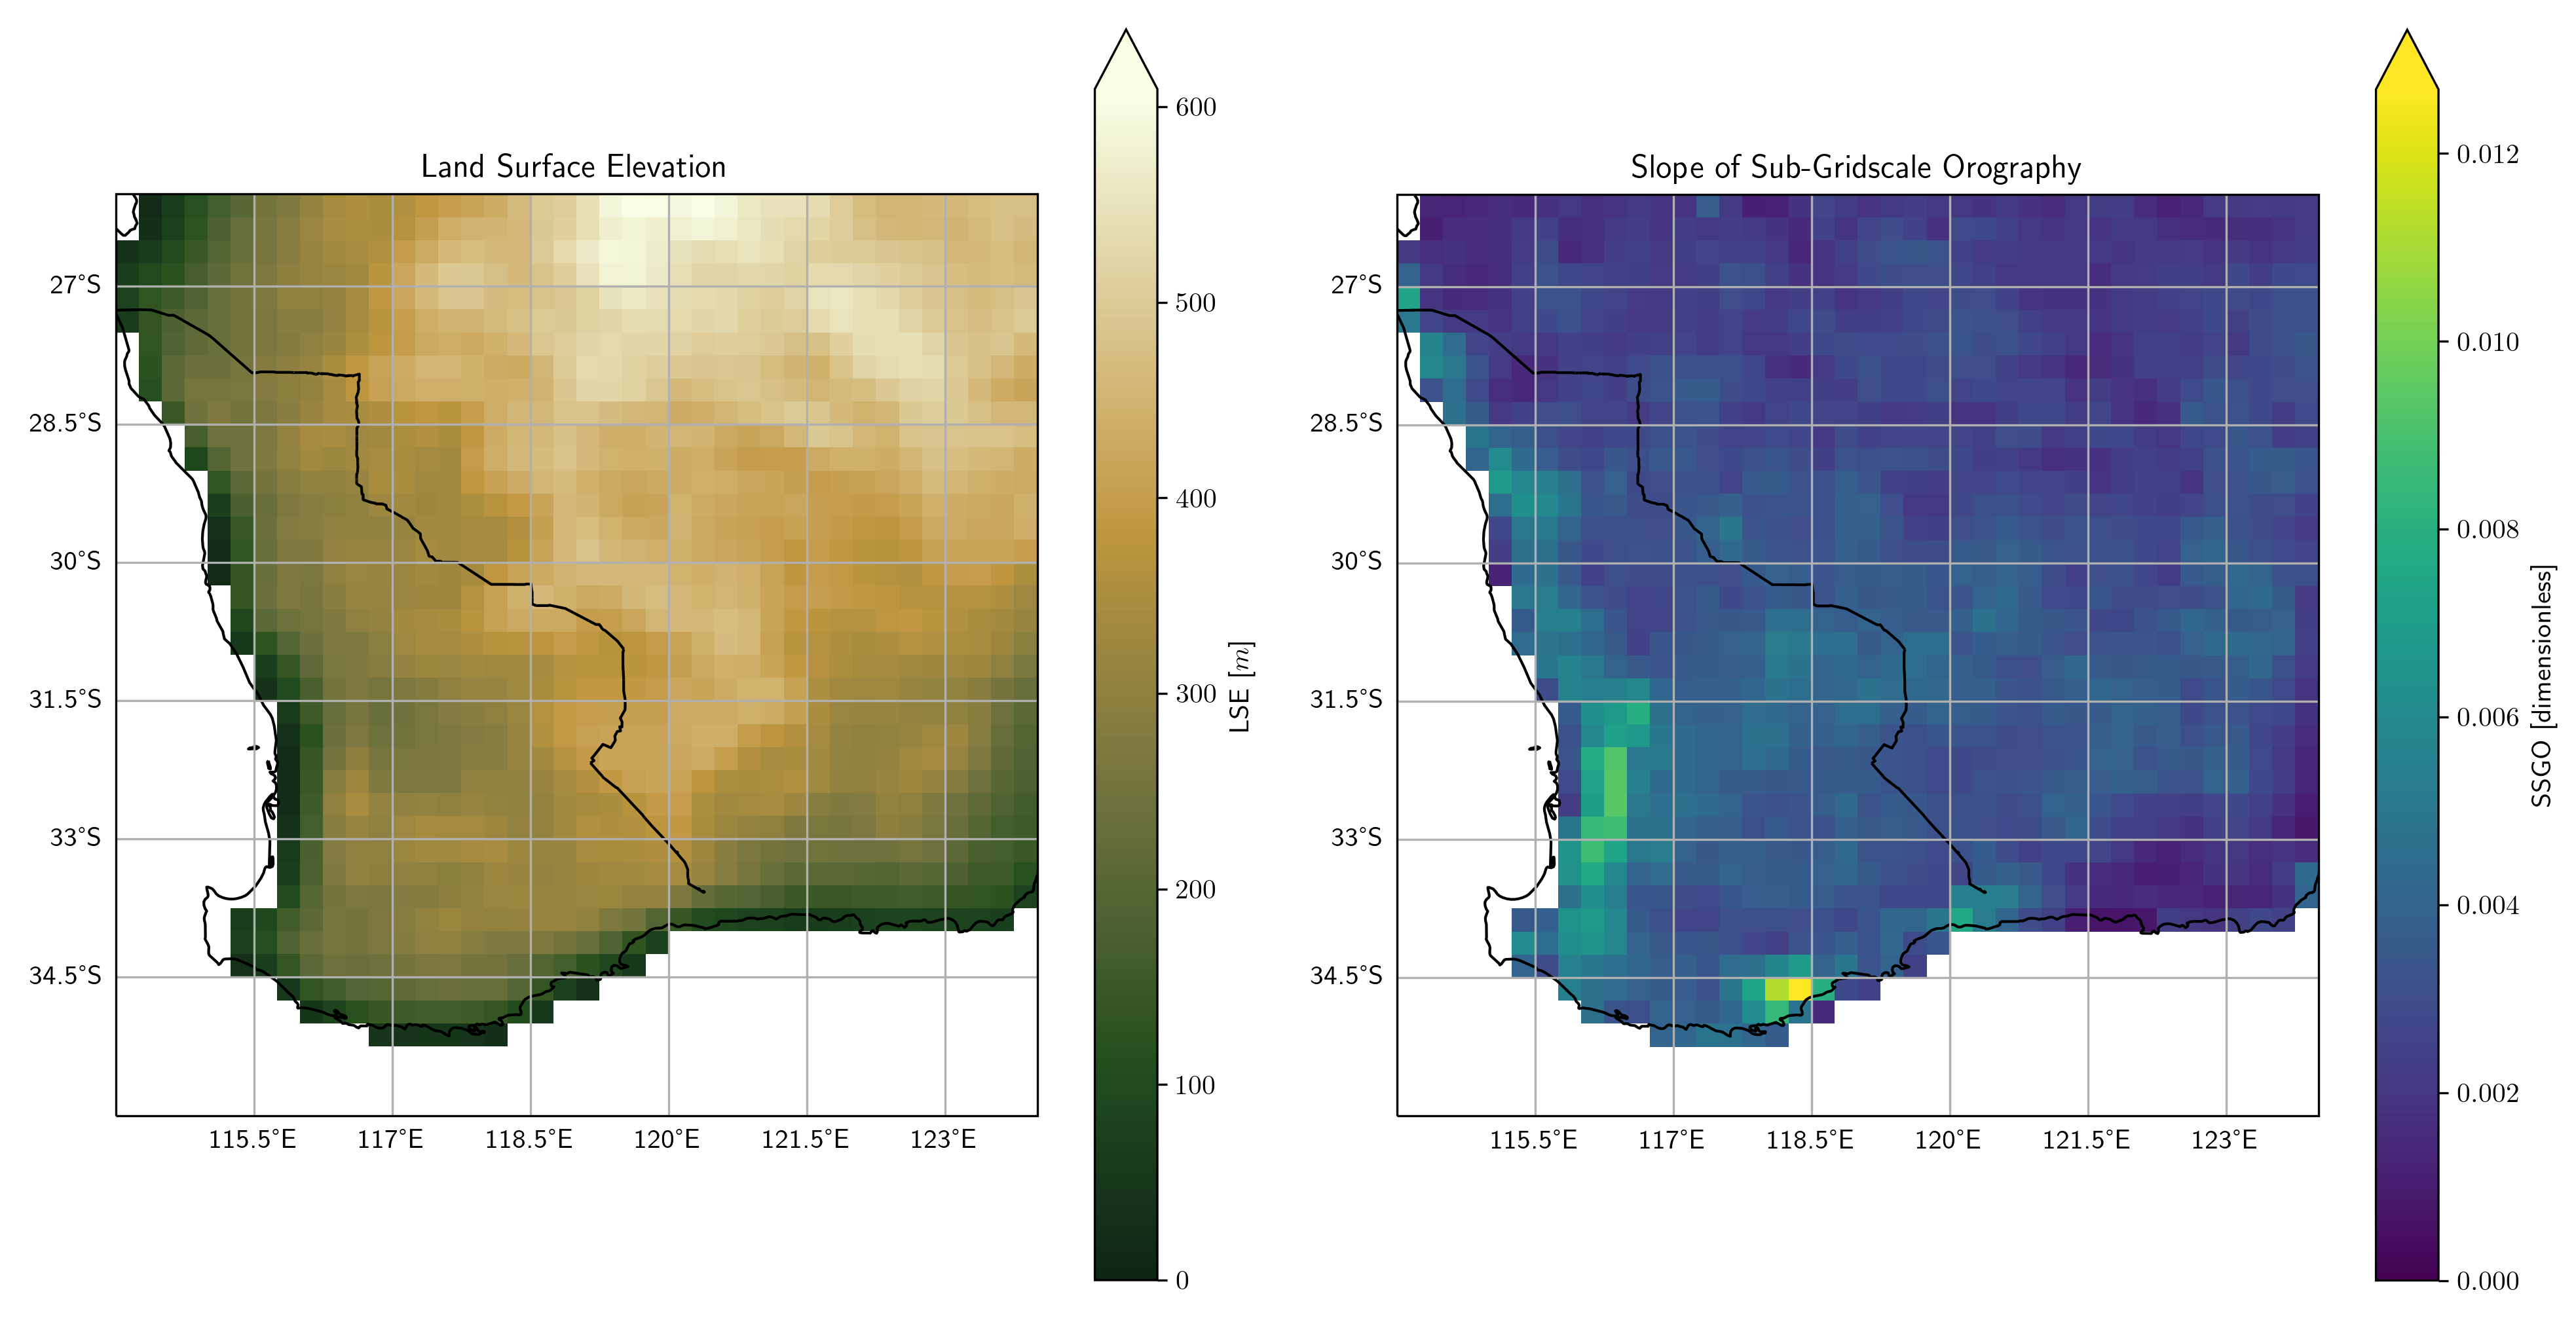
\includegraphics[width=0.9\textwidth]{wa_orog.png}
	\caption[Orography for WA focus region]{\acf{LSE} (left) and \acf{SSGO} (right) for the \ac{WA} focus region.}
	\label{fig:wa_orog}
\end{figure}

\section{Diurnal comparison for January mean}
\label{sec:comp_diurnal}

\subsection{VIEC delineation along fence}

\ac{VIEC} mean values computed over January displayed a marked distinction across the \acf{SBFWA}, with more strongly negative values on the native side of the fence during both the day and night (see Figure~\ref{fig:wa_jan_comb_1}).\footnote{The following results are also observed to varying degrees for the months of February, October, November and December, but we present January because this month displays these trends most distinctly.} During daytime, this also marks the distinction between positive \ac{VIEC} values on the agricultural side and negative values on the native side. Negative $\ac{VIEC}$ values indicate a greater prevalence for upwards air movement (kinetic energy converted into gravitational potential energy), while positive values indicate the opposite.\footnote{There are better variables than \ac{VIEC} in the ERA5 dataset to analyse upwards and downwards air movement since \ac{VIEC} lumps internal and gravitational potential energy together, but these other variables were not included in the original analysis and time constraints in this project did not allow for modification of the methodology. See Section~\ref{ssec:era5_improve}.}

\begin{figure}[!ht]
	\centering
	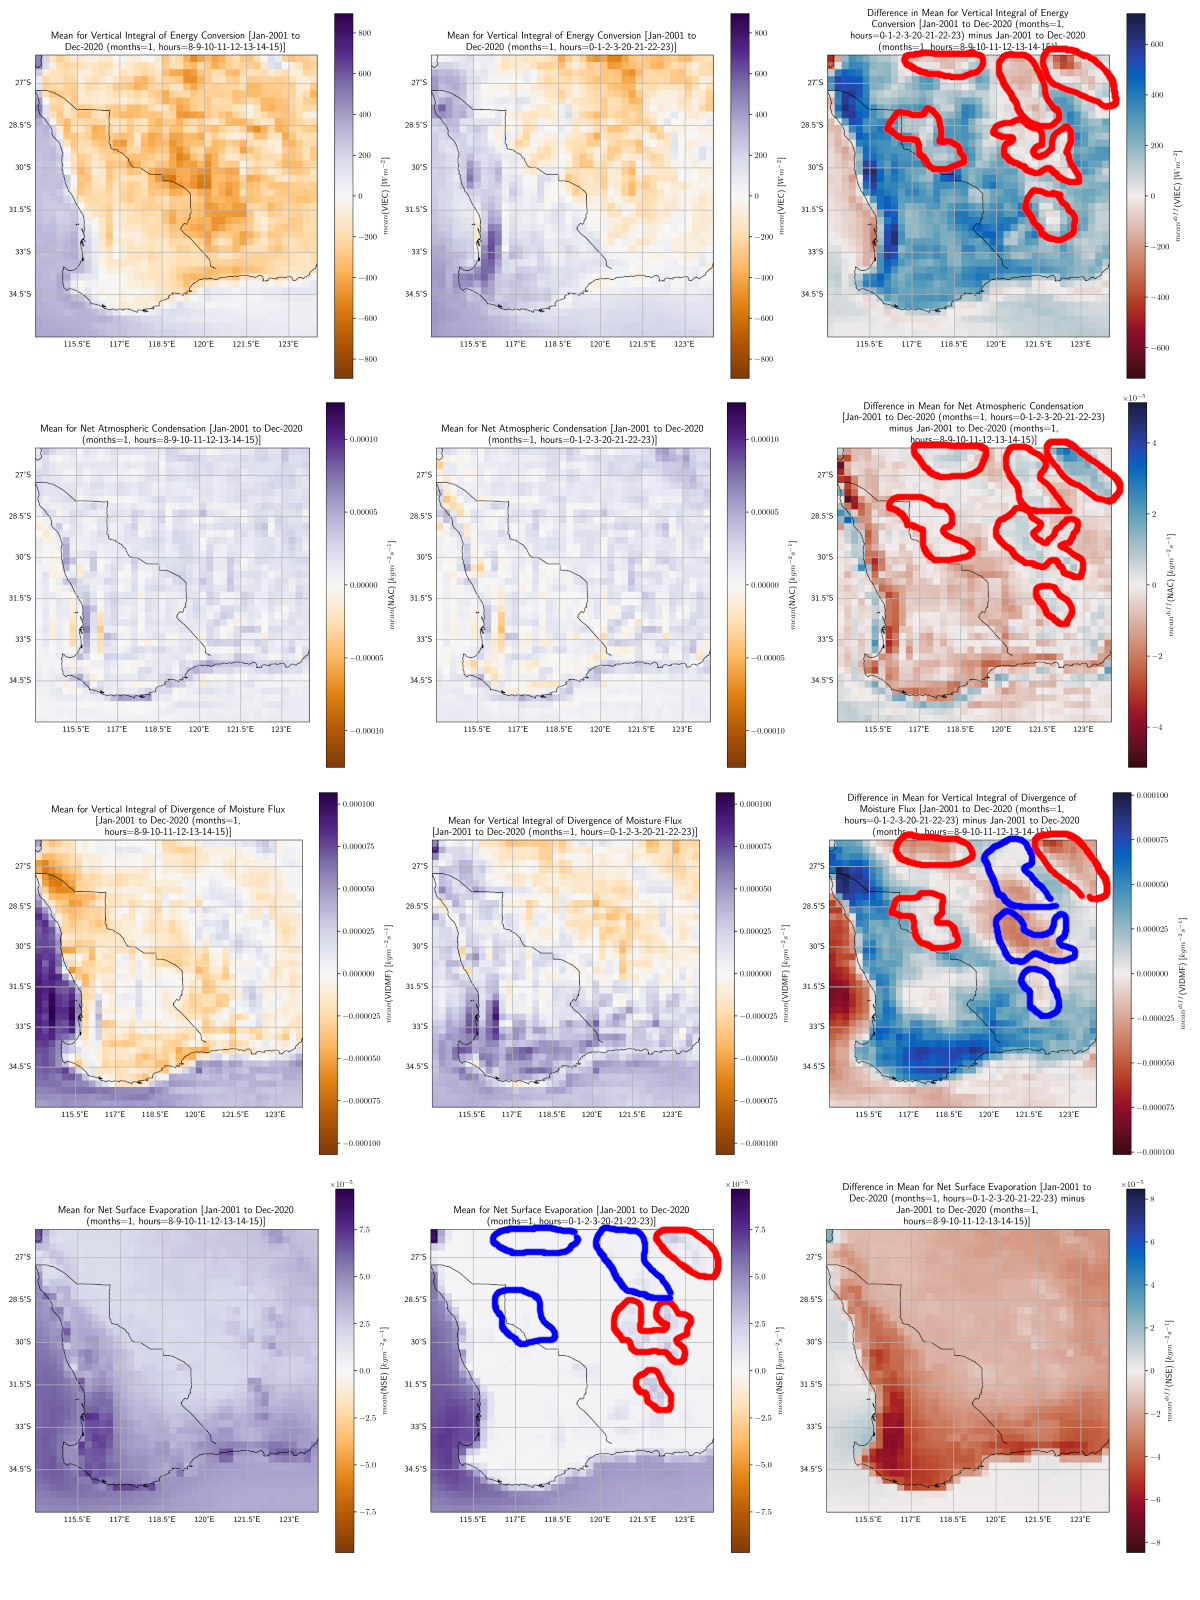
\includegraphics[width=0.9\textwidth]{wa_jan_comb_1.png}
	\caption[January means for selected variables 1]{January mean daytime and nighttime values for \acs{VIEC}, \acs{NAC}, \acs{VIDMF} and \acs{NSE}. Red markings indicate selected areas which are distinct from background trends. Blue markings indicate areas where such a distinction did not exist, but did exist for \acs{VIEC}.}
	\label{fig:wa_jan_comb_1}
\end{figure}

The large-scale patterns observed for \ac{VIEC}$^{diff}$ in arid \ac{WA} are mostly a reflection of warmer temperatures during daytime, and warmer temperatures on the native side due to thermal retention and lower albedo of native vegetation compared to bare agricultural soil in January. Evidence for this is a remarkable large-scale spatial correlation between \ac{T2}, \ac{MSLP} and \ac{VIEC} for all months of the year (not shown, but January results are displayed in Figure~\ref{fig:wa_jan_comb_2}). This suggests that the large-scale tendencies for vertical air mass movements in inland areas\footnote{Coastal effects are treated separately in Section~\ref{sec:comp_seasonal_1400}.} are driven by surface heating, in accordance with standard theory.

\begin{figure}[!ht]
	\centering
	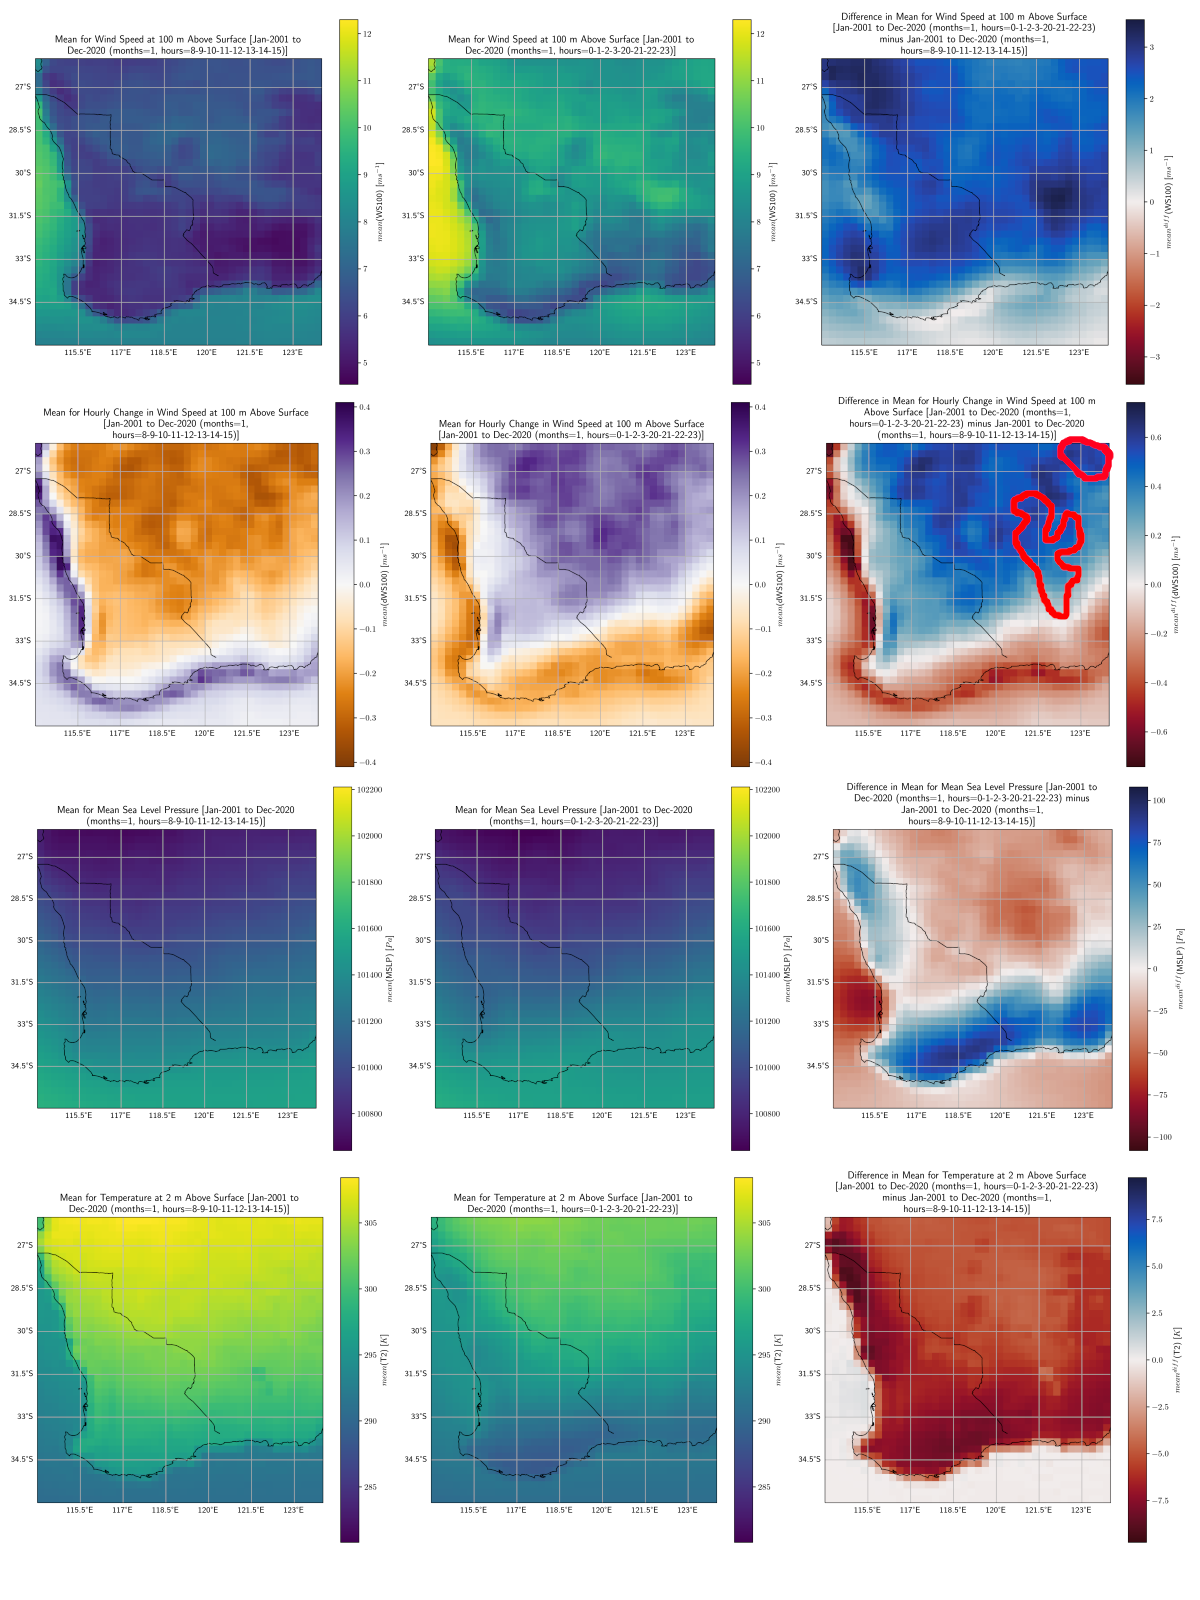
\includegraphics[width=0.9\textwidth]{wa_jan_comb_2.png}
	\caption[January means for selected variables 2]{January mean daytime and nighttime values for \acs{WS100}, \acs{dWS100}, \acs{MSLP} and \acs{T2}. Red markings indicate selected areas for \acs{dWS100} which are distinct from background trends but which deviate from orographic spatial patterns.}
	\label{fig:wa_jan_comb_2}
\end{figure}

\subsection{Localised anomalies}

However, there are local-scale features which act contrary to this background trend. These are highlighted with red markings in Figure~\ref{fig:wa_jan_comb_1}.\footnote{The use of coloured markings with a thick outline somewhat distorts perception of these features. For an unmarked version of the figure, see Appendix~\ref{sec:unmarked}.} In these areas, \ac{VIEC} becomes increasingly negative (air movements are increasingly upwards directed) from daytime to nighttime despite the decrease in temperature, and there did not appear to be any localised anomalies in \ac{T2} which could explain this (see Figure~\ref{fig:wa_jan_comb_2}).

Interestingly, these \ac{VIEC}$^{diff}$ anomalies correspond to localised areas of positive \ac{NAC}$^{diff}$ (see Figure~\ref{fig:wa_jan_comb_1}). Given the suspected role of \ac{CIAD}, we turn to the question of whether this correlation primarily reflects a chance convergence of winds manifesting stronger upwards air movements which was then conducive towards cloud formation, or whether the actual condensation itself was responsible for the strengthening vertical motions.

\subsection{Contribution from lake evaporation}

At least a few of these anomalies can be attributed to evaporation from ephemeral lakes\footnote{Although ephemeral, use of Google Earth satellite images confirms that these lakes contained water for all December months within the study period (and the water is presumably still there by January).}, which calls into question how relevant chance wind convergence would be on top of this. The lakes display a relatively low magnitude of evaporation decrease going from daytime to nighttime temperatures. This can be seen in the difference plot (right column) for \ac{NSE} in Figure~\ref{fig:wa_jan_comb_1} but for visual clarity, these lakes were marked in red for the nighttime plot (middle column) instead.

Furthermore, given the low magnitude of \ac{NSE} over these lakes relative to background trends, we would have expected increased water vapour \textit{divergence} via diffusion (positive \acs{VIDMF}$^{diff}$). But instead, what we observe is that these lakes correspond to areas of \textit{negative} \acs{VIDMF}$^{diff}$ (indicating increased water vapour \textit{convergence}). Given it is unlikely for a chance convergence of winds to coincidentally conform to the extents of the lakes, this flags the possibility of \ac{CIAD} as to our knowledge there has been no other proposed mechanism which would explain this anomaly. That is, continued evaporation combined with cooler temperatures during night time leads to increased atmospheric condensation, and under this may form a localised area of low pressure which advects air and moisture towards itself for sustenance.

\subsection{Implications for surface wind resource} 

In studying implications for wind energy generation, we turn towards 100 m wind speed (\acs{WS100}) as well as the \textit{hourly change} in 100 m wind speed (\acs{dWS100}). The latter allows us to analyse effects upon \acs{WS100} which may be slight and difficult to visually identify from a plot of \ac{WS100} itself since the signal is dominated by synoptic effects.

\subsubsection{WS100 higher on native side of fence}

Despite lower roughness on the agricultural side of the fence in January (when there is no crop and often bare soil), \ac{WS100} is higher on the native side of the fence and shows some signs of being delineated along the fence itself. This is likely a reflection of surface air pressure differences arising from temperature differences (see Figure~\ref{fig:wa_jan_comb_2} left and middle columns; note how the fence delineations for \ac{WS100}, \ac{MSLP} and \ac{T2} do not hold along the southern part of the region from 34.5$^\circ$S to 31.5$^\circ$S). Given that results for \ac{T2} shows a clear demarcation along the fence in Figure~\ref{fig:wa_jan_comb_2}, it then follows that wind speed variations beyond the effect of surface roughness can in part be attributed to the type of vegetation cover. Future changes to vegetation cover (such as eastward agricultural expansion, or change in crops being grown) which cause a decrease in temperatures may possibly reduce wind speeds (and the converse for increases in temperature).

\subsubsection{Anomaly for diurnal difference in MSLP on native side of fence}

\paragraph{Decrease in pressure despite convergence of mass and decrease in temperature}

Although the spatial pattern observed for \ac{MSLP}$^{diff}$ is similar to that of \ac{T2}$^{diff}$ in Figure~\ref{fig:wa_jan_comb_2}, a large area of the focus region (mostly on the native side of the fence) sees a \textit{decrease} in surface pressure going from day to night despite a decrease in temperature. So mass flux directed away from the surface of this area (i.e.\ decreasing surface pressure) does not appear to be caused by surface temperature changes inducing \textit{upwards} air movement. Nor does it appear to be caused by \textit{outwards} (horizontal) mass transport given that much of this area displays increased moisture \textit{convergence} (negative \acs{VIDMF}$^{diff}$) in Figure~\ref{fig:wa_jan_comb_1} (in turn implicating increasing \textit{convergence} of winds and air mass in general).

\paragraph{Possible explanations}

The remaining explanations are either that there is some climate feature in the upper atmosphere or outside of this focus region or which interacts with the surface of this focus region to produce a reduction of pressure towards nighttime, or that the reduction in surface pressure actually arises from a drop in air density as gaseous water condenses out as liquid.

The latter appears to only be mildly supported by the \ac{NAC} results in Figure~\ref{fig:wa_jan_comb_1}. An increase of condensation only occurs in certain parts of the area where there is negative \ac{MSLP}$^{diff}$, and these parts do correlate with especially negative \ac{MSLP}$^{diff}$ values, but it is not clear whether these distributed localisations of condensation can produce the area-scale effect seen for \ac{MSLP}$^{diff}$. However, it should be noted that much of the patchiness observed in \ac{NAC} could possibly result from the fact that \ac{NAC} is a hybrid value derived a mixture of instantaneous and accumulated \ac{ERA5} variables (see Appendix~\ref{sec:nac_derive}).

\paragraph{Possible implications for surface wind}

If it is indeed the case that atmospheric condensation is responsible for the surface pressure drop and hence increase in wind speeds, then this is yet another mechanism by which the surface wind resource depends on land cover, given results by \citep{lyons2002, ray2003} which clearly demonstrates that land cover modulates cloud formation preferences (also see Section~\ref{ssec:native_nac}).

\subsubsection{Anomalies in dWS100}

\paragraph{dWS100 correlated with LSE, VIEC and NAC}

The spatial pattern observed for \acs{dWS100} corresponds mostly to the \ac{LSE} displayed in Figure~\ref{fig:wa_orog}. Higher elevations are correlated with more negative d\ac{WS100} values during the daytime, more positive values during nighttime, and hence a greater magnitude of increase from day to night. Selected areas which display the opposite trends are highlighted with red markings in Figure~\ref{fig:wa_jan_comb_2}.\footnote{For an undistorted view, see the figure without markings in Appendix~\ref{sec:unmarked}.}

Interestingly, these areas correspond with the lakes identified earlier, and actually show an especially positive value for \acs{dWS100}$^{diff}$ (strengthening of winds). A more negative \ac{VIEC}$^{diff}$ (less conversion of internal and gravitational potential energy to kinetic) in these areas should imply a more negative \acs{dWS100}$^{diff}$ (weakening of winds) all other things equal, so it is not clear what is causing this anomaly. One possibility is that convection associated with increased \ac{NAC} (cloud formation) in these areas at nighttime lead to favourable energy exchanges between the boundary layer and free atmosphere, and a reversal of this effect in the daytime manifests as a greater decrease in wind speed.

\paragraph{Possible implications for surface wind}

If it can be shown that positive \ac{NAC}$^{diff}$ consistently correlates with especially positive \ac{dWS100}$^{diff}$, then land cover is again implicated through land cover modulation of cloud formation, with the effect that native vegetation induces a greater ramp rate in wind speeds in summer (when clouds preferentially form over the native side of the fence).

\section{Seasonal comparison for 1400 mean}
\label{sec:comp_seasonal_1400}

\subsection{Seasonal difference in MLAI}

Figure~\ref{fig:wa_lai_seasonal} displays a comparison for the \acl{MLAI} between the months of \ac{JJA} and \ac{DJF}. Native vegetation on the east of the \ac{SBFWA} show negligible differences. There is a significant loss in \ac{MLAI} towards the \ac{DJF} months as the wheat and barley crops which were grown from May to November are harvested in November \citep{lyons1996}. The extents of the \ac{MLAI} loss correspond well with the Wheat Belt region of Western Australia (see Figure~\ref{fig:lc_wa}). Slight (relative to \ac{JJA} base value) greening appears to occur in the coastal Jarrah forests through the spring and summer months.

\begin{figure}[!ht]
	\centering
	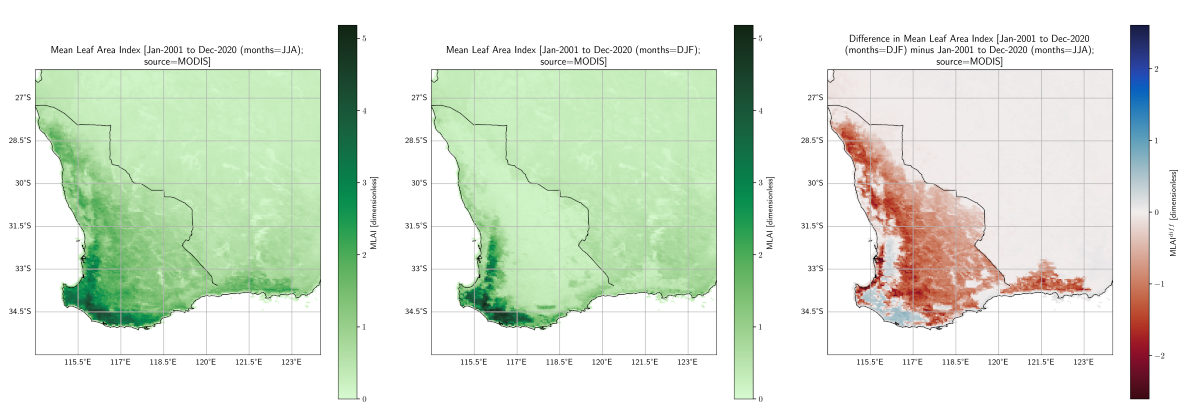
\includegraphics[width=0.9\textwidth]{wa_lai_seasonal.png}
	\caption[MLAI seasonal comparison for WA focus region]{\ac{MLAI} computed over \acs{JJA} and \acs{DJF} (left and middle), as well as the difference in these values between the two seasons (right).}
	\label{fig:wa_lai_seasonal}
\end{figure}

\subsection{Correlation between VIEC and NAC}

\ac{VIEC} mean values computed over 1400 \ac{LT} display a remarkable spatial correlation with that of \ac{NAC}. This is especially apparent near the coast for \ac{JJA} means, and in general for the difference plots between \ac{JJA} and \ac{DJF} (leftmost and rightmost columns in Figure~\ref{fig:wa_14_comb_1} respectively). More positive \ac{NAC} and \ac{NAC}$^{diff}$ values are correlated with more negative \ac{VIEC} and \ac{VIEC} $^{diff}$ values respectively. \ac{T2}$^{diff}$ (see Figure~\ref{fig:wa_14_comb_2}) shows a relatively uniform pattern and is consistent with the large-scale trend in \ac{VIEC} $^{diff}$ (warmer air tends to rise more), but it does not capture any of the smaller-scale trends that \ac{NAC}$^{diff}$ does.

\begin{figure}[!htp]
	\centering
	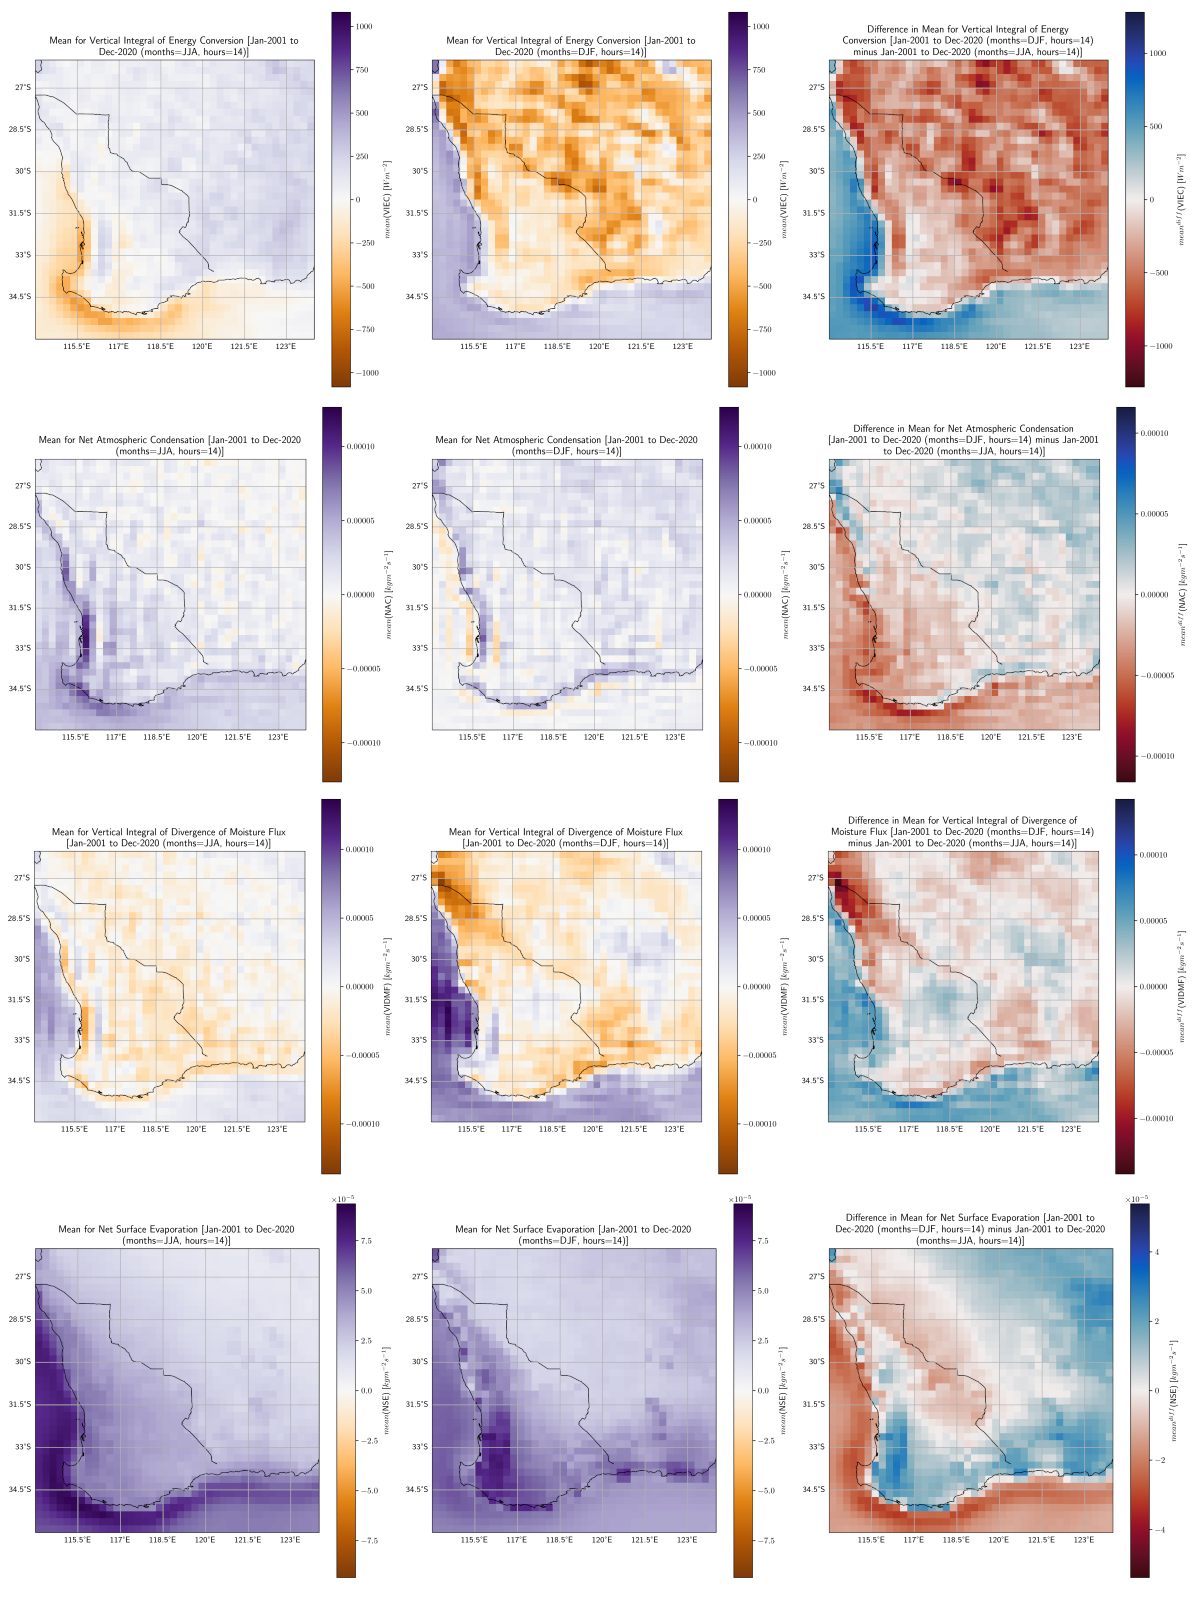
\includegraphics[width=0.9\textwidth]{wa_14_comb_1.png}
	\caption[1400 means for selected variables 1]{1400 mean \acs{JJA} and \acs{DJF} values for \acs{VIEC}, \acs{NAC}, \acs{VIDMF} and \acs{NSE}.}
	\label{fig:wa_14_comb_1}
\end{figure}

\begin{figure}[!htp]
	\centering
	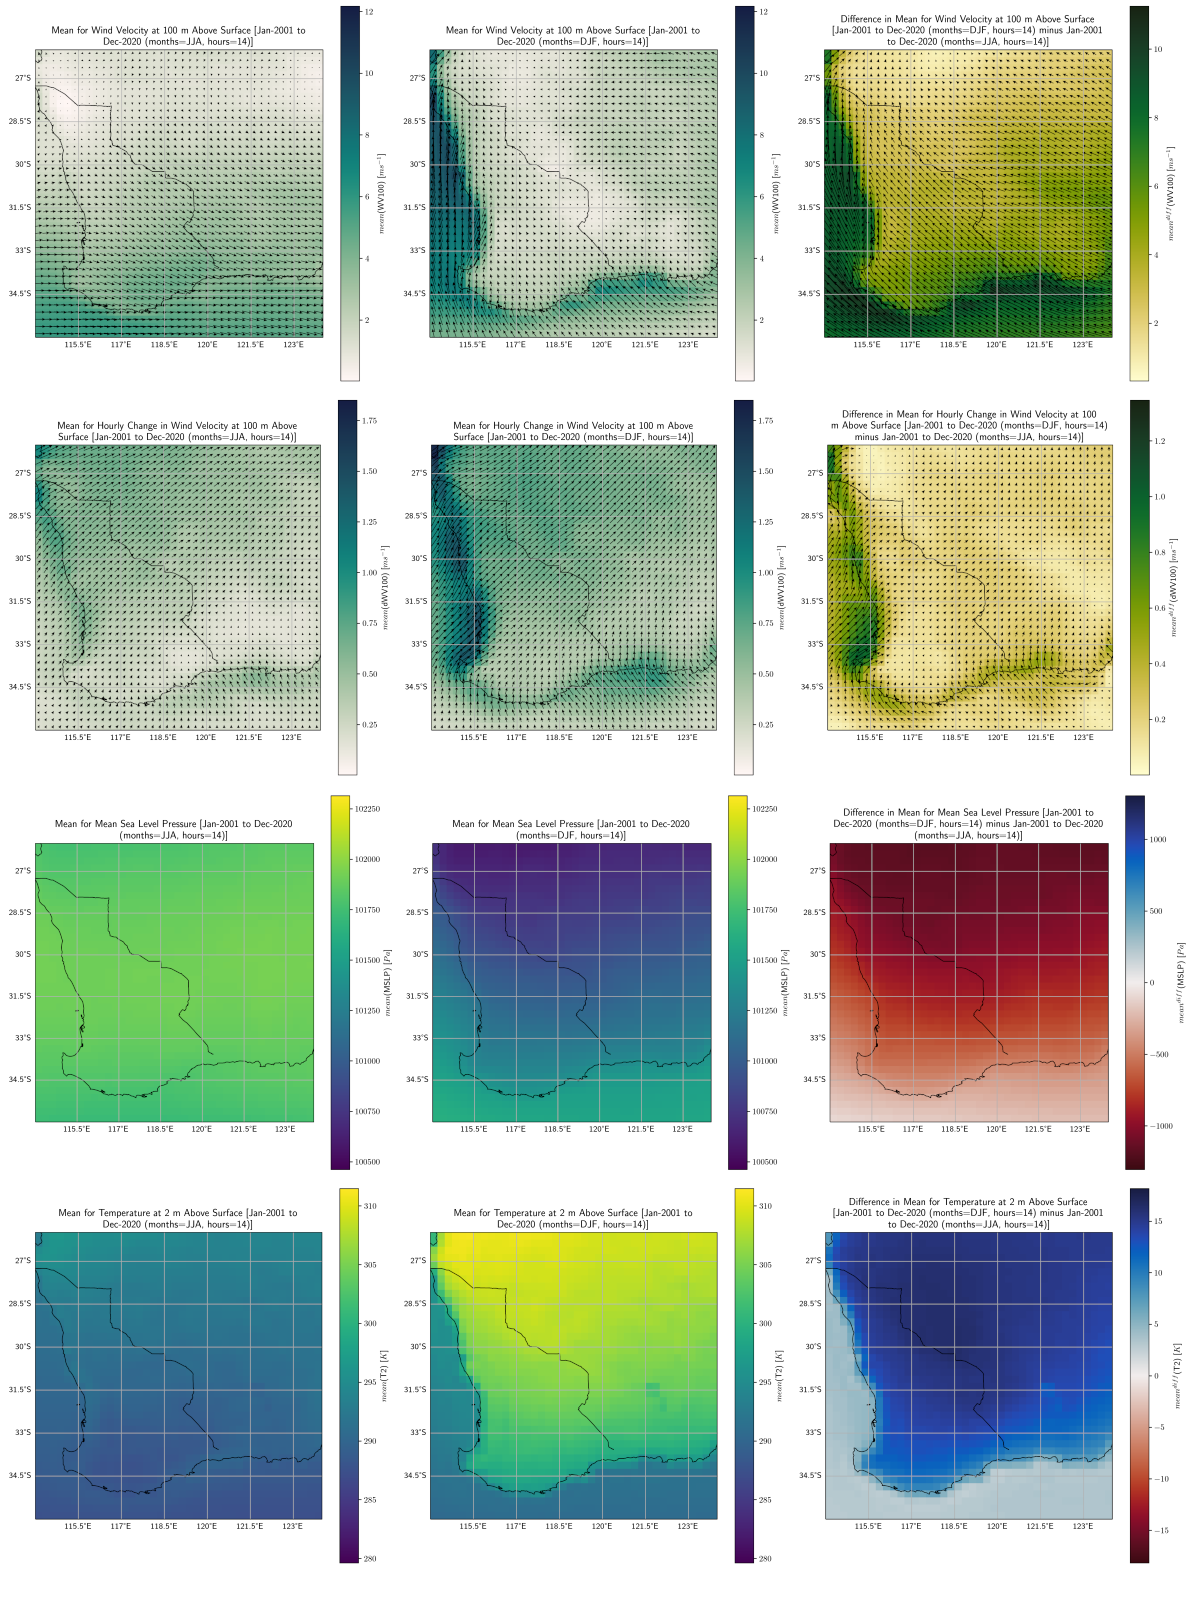
\includegraphics[width=0.9\textwidth]{wa_14_comb_2.png}
	\caption[1400 means for selected variables 2]{1400 mean \acs{JJA} and \acs{DJF} values for \acs{WV100}, \acs{dWV100}, \acs{MSLP} and \acs{T2}.}
	\label{fig:wa_14_comb_2}
\end{figure}

We choose to display results for 1400 \ac{LT} here because results for this hour are most distinct, but the following is actually more or less observed for all hours of the day in the hourly means analysis and all months of the year in the monthly means analysis (not shown):
\begin{itemize}
	\item For both \ac{JJA} and \ac{DJF} results, we observe that on the native side of the fence, most areas of negative \ac{VIDMF}$^{diff}$ (increased moisture \textit{convergence}) correlate with areas of positive \ac{NSE}$^{diff}$ (increased evaporation) but positive \ac{NAC}, contrary to what is expected from diffusion but consistent with \ac{CIAD}.
	\item None of the variables from which \ac{NAC} is derived display similar local-scale spatial variations to \ac{VIEC} across most of the focus region (\ac{VIDMF} and \ac{NSE} for 1400 are displayed in Figure~\ref{fig:wa_14_comb_1}, \ac{TCWV} not shown at all). Only \ac{NAC} itself is similar to \ac{VIEC}.\footnote{Exceptions occur for hours 0500-0700 \ac{LT} and 1700-1900 \ac{LT} due to data artefacts in \ac{ERA5}, but this should not affect the conclusions. See Appendix~\ref{sec:artefact} for discussion.}
	\item The concentrated band of negative \ac{VIEC} and positive \ac{NAC} means along the southwestern coastline for \ac{JJA} is present regardless of whether the band is upwind or downwind of the coastline, and whether the temperature gradients are producing a land or sea breeze (see \ac{T2} and \ac{dWV100} in Figure~\ref{fig:wa_14_comb_2} for 1400 \ac{LT} results).
\end{itemize}

The final point indicates that coastal orography and differential heating are unlikely to be responsible for the concentrated band along the southwestern coastline. And these points together conspire to heavily implicate the possibility of \ac{CIAD}.

\subsection{The role of coastal geography}

One way in which negative \ac{VIEC} (rising air) could theoretically be concentrated along the coastline is if low-lying oceanic winds experience a sudden change in surface elevation and are deflected upwards from coastal cliffs and urban structures. But this does not explain why the observed bands in Figure~\ref{fig:wa_14_comb_1} extends out into the oceans, nor why the band is observed on the southernmost part of this region (around 35$^\circ$S) where winds are blowing from relatively high terrestrial ground to relatively low ocean surface (see \ac{WV100} in Figure~\ref{fig:wa_14_comb_2}). Furthermore, much stronger winds are blowing onshore during the \ac{DJF} months yet this coastal band is not observed for these months (compare \ac{VIEC} in Figure~\ref{fig:wa_14_comb_1} with \ac{WV100} in Figure~\ref{fig:wa_14_comb_2}). So it seems extremely unlikely that coastal orography is the cause.

\subsection{The role of coastal differential heating}

Another way in which negative \ac{VIEC} (rising air) could theoretically be concentrated along the coastline is if a localised pressure gradient (arising from a temperature gradient) along the coastline adverse to the wind direction caused a bunching up of mass such that air had to be directed upwards. But results indicate the presence of this band regardless of the strength and direction of the coastline temperature gradient relative to prevailing winds. For the case of 1400 \ac{LT}, Figure~\ref{fig:wa_14_comb_2} displays a negligible coastal pressure gradient, temperature gradient and magnitude of \ac{dWV100} in \ac{JJA}, yet the band exists for these months but not \ac{DJF} where these parameters are much more significant. So it also seems highly unlikely that differential heating is the cause.

Although Figure~\ref{fig:wa_14_comb_2} displays a negligible coastal gradient in \textit{air} temperature for \ac{JJA} at 1400 \ac{LT}, the Leeuwin (Ocean) Current during these months actually brings about a significant increase in \ac{SST} for the continental shelf waters \citep{berthot1997}. This can be seen in Figure~\ref{fig:wa_14_comb_1}, where offshore evaporation is significantly higher in \ac{JJA} than \ac{DJF} despite lower solar irradiance.

\subsection{The role of coastal condensation}
\label{ssec:coastal_cond}

\subsubsection{Atmospheric condensation as cause for convective initiation}

\paragraph{Summary of conclusions from seasonal comparison thus far}

In summary, the coastal concentration of negative \ac{VIEC} (upwards air movements) occurs in continental shelf waters where \textit{air} temperature is comparable to that on land, but where \textit{water} temperatures are higher than that of air due to the winter presence of the Leeuwin Current. There is additional atmospheric moisture from the warmer waters which contributes to air buoyancy but analysis of \ac{CAPE} values reveals no coastal concentration whatsoever (not shown).\footnote{This is in spite of the fact that \ac{CAPE} in the \ac{ERA5} dataset is known to occasionally give unrealistically high values \citep{ecmwf}.} So having ruled out mechanical deflection of winds from coastal geography, localised pressurisation from coastal differential heating, higher offshore \textit{air} temperatures leading to upwards thermal expansion, and additional air buoyancy from increased atmospheric moisture, \ac{CIAD} is to our knowledge the only proposed mechanism consistent with the results.

\paragraph{Direction of causation}

In the \ac{CIAD} picture, additional winter atmospheric moisture from the Leeuwin Current is conducive towards coastal cloud formation, and it is this atmospheric condensation (positive \ac{NAC}) which initiates convection and subsequent uplift of air (negative \ac{VIEC}). That is, the direction of causation for \textit{initiation} of local circulations is from condensation to convection. In the ensuing circulation, the direction of causation is ill-defined as there is a positive feedback loop between the two. The circulation persists until the available moisture (latent energy) is unable to sustain the air motions.

\subsubsection{Interactions with temperature gradients and surface energy fluxes}
\label{ssec:nac_t2}

On top of this, there is the effect of coastal temperature gradients in determining the spatial distribution of atmospheric moisture available for condensation, and the effect of \ac{SSHF} inland in determining whether there is sufficient convective mixing for the \ac{BLH} to penetrate the \ac{LCL} for condensation to occur.

\paragraph{Consistency with JJA results}

Weaker winds from temperature gradients in \ac{JJA} compared to \ac{DJF} means the buildup of oceanic moisture along the coasts has a high condensation rate relative to moisture convergence flux to inland areas. For the 1400 \ac{LT} case, this is reflected in \ac{JJA} by low \ac{WV100} magnitude, low \ac{dWV100} magnitude and weak coastal \ac{T2} contrast in Figure~\ref{fig:wa_14_comb_2}, as well as a less positive \ac{VIDMF} offshore (west of the coastline) despite higher \ac{NSE} in Figure~\ref{fig:wa_14_comb_1}. The result is that \ac{VIEC} displays a similar band to \ac{NAC} along the coast. This is also supported by the fact that the negative \ac{VIEC} band is absent from around 29$^\circ$S to 27$^\circ$S, which coincides with where \ac{dWV100} is especially strong.

\paragraph{DJF results and flux of moisture convergence towards fence}

On the other hand, stronger winds from temperature gradients in \ac{DJF} imply the converse. The ratio of inland moisture flux transport to coastal condensation rate is relatively high (in part due to lower coastal moisture from absence of Leeuwin Current), so no coastal band of negative \ac{VIEC} is observed. Instead, there is increased condensation (relative to \ac{JJA}) on the native side of the fence, possibly due to higher \ac{SSHF}, and this is where negative \ac{VIEC} concentrates instead. This would seem to be supported by \ac{VIDMF} results which show for \ac{DJF} how moisture convergence (negative \ac{VIDMF}) moves inland ahead of moisture divergence (positive \ac{VIDMF}) as the day progresses, eventually reaching a point where convergence is concentrated on the native side of the fence (see Figure \ref{fig:wa_vidmf}).

\begin{figure}[!htp]
	\centering
	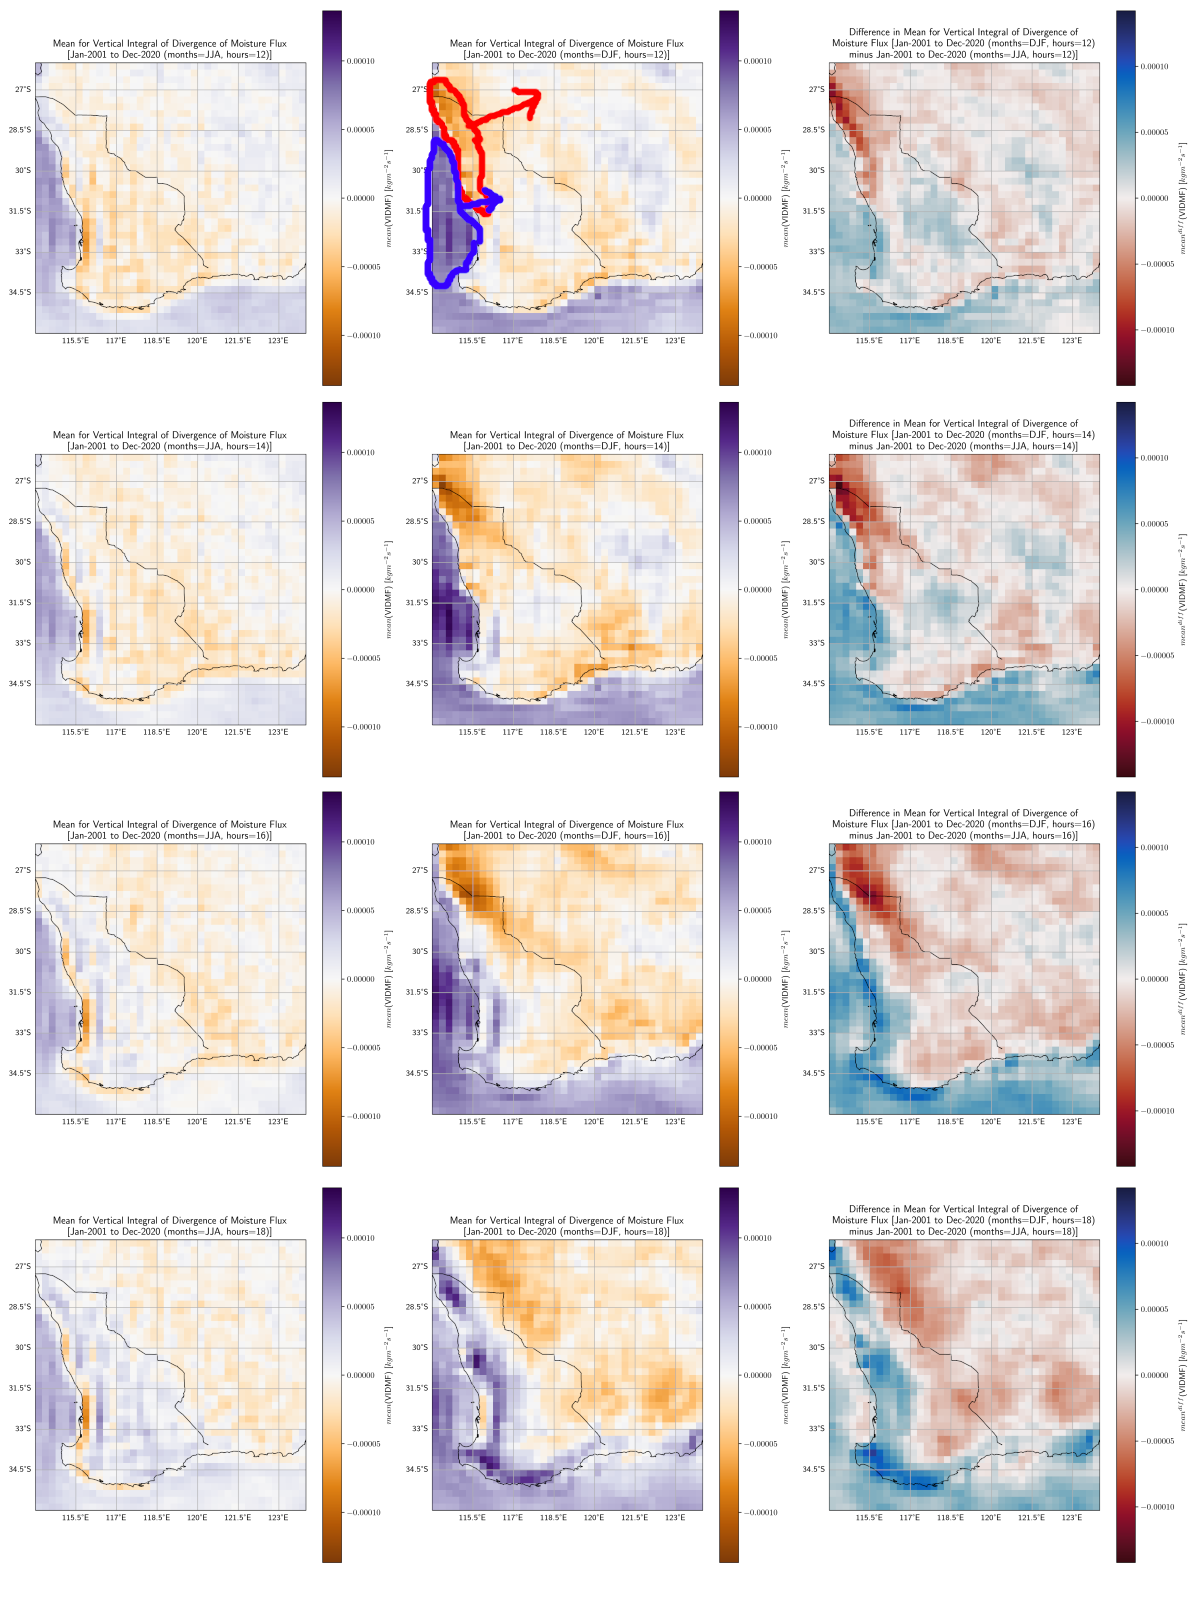
\includegraphics[width=0.9\textwidth]{wa_vidmf.png}
	\caption[1200-1800 means for VIDMF]{1200-1800 mean \acs{JJA} and \acs{DJF} values for \acs{VIDMF}. Red and blue markings illustrate how moisture convergence and divergence respectively is initially concentrated near the coastline then moves inland as the day progresses, eventually reaching a point where convergence is concentrated on the native side of the fence.}
	\label{fig:wa_vidmf}
\end{figure}

\subsection{Implications for surface wind resource} 
\label{ssec:implications}

\subsubsection{Effect on coastal breezes}

The replacement of native vegetation with annual crops, where there is irrigation in winter, bare cover after harvesting in summer, and lower albedo year round, has likely led to the lower surface temperatures observed on the western side of the \ac{SBFWA} year round. These lower temperatures were observed in the monthly means analysis for \ac{T2} (not shown) but can also be seen in Figure~\ref{fig:wa_14_comb_2} for the case of 1400 \ac{LT} in \ac{DJF}. Assuming that native vegetation cover which existed in the southwest region prior to agricultural clearing had similar temperatures to that currently observed on the native side of the fence, diurnal monthly means analysis (not shown) suggests that the agricultural clearing has led to:
\begin{itemize}
	\item For daytime during warmer months (Oct to Mar): a weakening of the sea breeze
	\item For nighttime during warmer months (Oct to Mar): a slight strengthening of the land breeze, with possibly a reversal from slight sea breeze to slight land breeze
	\item For daytime during cooler months (Apr to Sep): a slight strengthening of the land breeze, with possibly a reversal from slight sea breeze to slight land breeze
	\item For nighttime during cooler months (Apr to Sep): a very slight strengthening of the land breeze
\end{itemize}

\subsubsection{Inland drying and coastal flooding}

In all cases this points towards a loss in inland atmospheric moisture, and may partly explain the well documented loss of rainfall and water vapour in the southwest region \citep{gordon2003, narisma2003, pitman2004, junkermann2009}. To the extent that atmospheric moisture is oceanic in origin (as opposed to from plant transpiration), as is often the case given the coastal location and dry climate of this region, a corollary to reduced inland moisture flux is an increased flood risk from the coastal buildup of moisture.

\subsubsection{Possible exacerbation under CIAD}

The available evidence appears to support the \ac{CIAD} framework moreso than it does the notion that cloud formation is a passive byproduct of moist air masses rising (whether due to surface heating, orography or chance convergence of winds). This is unless there is some systematic error in the \ac{ERA5} dataset which we are not aware of and which just so happens to produce misleading results.

Assuming this isn't the case and also assuming that the \ac{CIAD} framework is valid, then beyond ocean-land temperature differences from native vegetation clearing there would have been an additional contribution from reduced atmospheric condensation. That is, the drop in air pressure which accompanies atmospheric condensation becomes less prevalent, so even less air and moisture is advected inland. And the result is further exacerbation to inland rainfall loss and coastal flood risk.

\subsubsection{How this affects wind energy operation}

\paragraph{Operational revenue and risk}

The strengthening and weakening of breezes has a direct impact on how much energy coastal wind farms are able to generate. Coastal breeze changes appear to only be slight except in the case of daytime during warmer months (Oct to Mar). These months also happen to be when energy demand from air conditioning is at its highest so all other things equal, this translates to a loss in wind generation revenue compared to if current agricultural cover was instead native vegetation cover. This is especially so since a weakening of the sea breeze also means less cool relief for the urban centre of Perth.

Coastal flooding also constitutes a tail risk for wind energy operation. There is obvious damage that can be done to both turbine structures as well as accompanying electrical infrastructure. Despite the context of continued climate change, such increases in risk might not yet be internalised within project costs. Failure to properly capture these risks may produce losses which deter future investment.

\paragraph{Future changes in land cover}

There is further risk embodied within uncertainty of what future land cover will be. Afforestation efforts are a real possibility given increasing environmental consciousness by the public. Changing geopolitical-economic conditions, climate and public favour may also give way to the growing of different crops (including summer crops) in this region. Continued agricultural expansion is another possibility. In all these cases, it matters what species of trees or crops are being grown and how, as this determines the subsequent surface energy fluxes, temperature, and roughness.

Large-scale coastal afforestation using eucalypts with low albedo and high \ac{SSHF}, for example, are likely to strengthen the summer daytime sea breeze due to higher coastal temperatures (but it is unclear how sustainable this will be without the appropriate matter flux feedbacks (e.g.\ water, nutrients) granted by appropriate biodiversity). The large-scale adoption of summer crops with irrigation on the other hand, is likely to weaken the summer daytime sea breeze due to lower inland temperatures.

\paragraph{Possible changes in turbulence and condensation hotspots}

If \ac{CIAD} is valid, then the previous comments apply even more so. This also implies that land cover determines the concentration and spatial distribution of turbulence from rising air masses (negative \ac{VIEC}) via atmospheric condensation (positive \ac{NAC}). This in turn can introduce fatigue to turbine components and complex wake effects which inhibit energy generation. On top of this, future mining activity may change condensation hotspots and hence circulation patterns via changes in lake geochemistry affecting \ac{CCN} production \citep{junkermann2009}.

\section{Seasonal comparison for MDP statistics}

\subsection{Likely influence of agriculture on VIKE}

\subsubsection{Delineation along fence}

Figure~\ref{fig:wa_stats_seasonal_1} displays a delineation along the \ac{SBFWA} for $range$(\acs{VIKE}) and $hour_{max}$(\acs{VIKE}) in \ac{JJA}. None of the other \ac{MDP} statistics for \ac{VIKE} displayed remarkable results, and this spatial pattern may just be a coincidence. But the \ac{JJA} value for $range$(\acs{VIEC}) shows not only a delineation along the fence, but also along the edges of the coastal forests (compare with Figure~\ref{fig:wa_lai_seasonal}). However, this can also be interpreted as a coastal effect extending inland which is unrelated to the forests (it is difficult to distinguish between these since the forest cover follows the shape of the coastline).

\begin{figure}[!htp]
	\centering
	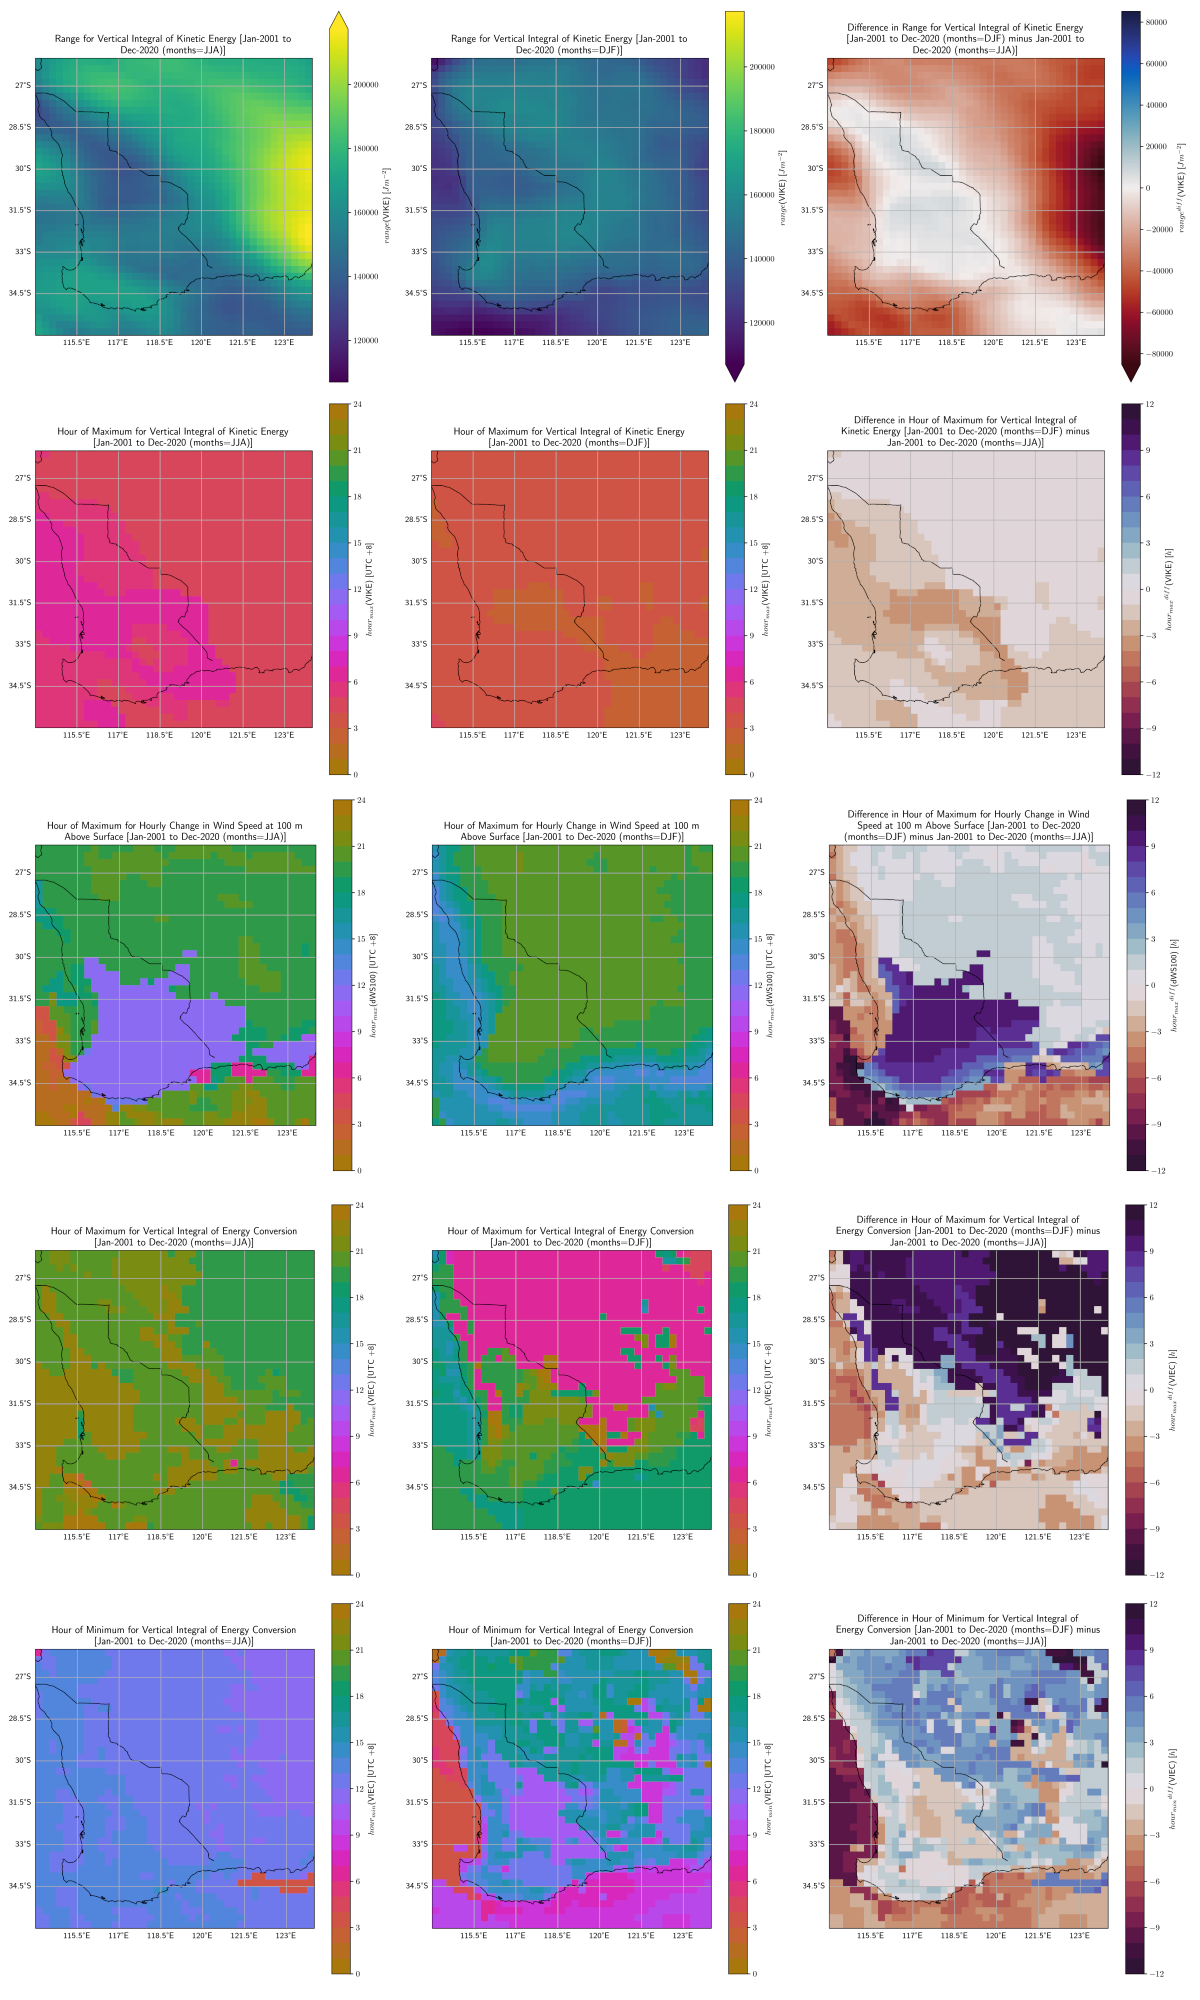
\includegraphics[width=0.75\textwidth]{wa_stats_seasonal_1.png}
	\caption[Selected MDP statistics with fence delineations]{Selected \ac{MDP} statistics (across various variables) which displayed delineations along the fence. Top to bottom: $range$(\acs{VIKE}), $hour_{max}$(\acs{VIKE}), $hour_{max}$(\acs{dWS100}), $hour_{max}$(\acs{VIEC}), $hour_{min}$(\acs{VIEC}).}
	\label{fig:wa_stats_seasonal_1}
\end{figure}

\subsubsection{Description of trends}

The \ac{JJA} values for \ac{VIKE} on the agricultural side show a smaller range, and an hour of maximum which is around two hours earlier. This is around the time of the morning boundary layer transition. \ac{VIKE} includes upper atmospheric air, so may be related to the surface via the boundary layer-free atmosphere interface. However, it is still unclear whether this is relevant and what is causing the observed spatial pattern. It is difficult to assess what effect cloud formation (which happens near the boundary layer-free atmosphere interface) might have, because \ac{NAC} is affected by assimilation cycle artefacts during these hours (see Appendix~\ref{sec:artefact}).

\subsubsection{Possible role of soil moisture}

Modelling by \citet{martius2021} suggests that soil moisture can have significant effects on the upper atmosphere. But to the extent that this is generally true of \acp{GCM}, the spatial pattern can also be interpreted as an artefact arising from sensitivities in the \ac{ECMWF} \ac{IFS} (which produces the \ac{ERA5} dataset). As \ac{VIKE} is a measure of \textit{horizontal} kinetic energy, this may affect the surface wind resource. But it is not clear how ($range$(\acs{WS100}) does \textit{not} show a similar pattern; not shown).

\subsection{Possible influence of agriculture on dWS100}

Figure~\ref{fig:wa_stats_seasonal_1} displays a somewhat marked distinction across the fence for $hour_{max}$(\acs{dWS100}) in \ac{JJA}. But the distinction does not sharply match the fence delineation. The results appear to suggest that wind speeds increase at the fastest rate around noon on the agricultural side and around the evening \ac{ABL} transition on the native side. $max$(\acs{dWS100}) displayed an increase from \ac{JJA} to \ac{DJF} over the entire region, with no obvious distinction across the fence (not shown). It is not known what is causing these results and whether this is reflecting an assimilation cycle artefact in \ac{ERA5} which we missed (see Appendix~\ref{sec:artefact}).

\subsection[Effect of native vegetation on VIEC diurnal phase]{Effect of native vegetation on phase of VIEC diurnal cycle}

\subsubsection{Minimum VIEC}

Figure~\ref{fig:wa_stats_seasonal_1} displays a delineation along the \ac{SBFWA} for $hour_{max}$(\acs{VIEC}) and $hour_{min}$(\acs{VIEC}) in \ac{DJF}. The bare agricultural cover in \ac{DJF} sees most negative \ac{VIEC} around noon, probably due to surface heating producing uplift of air. The native side sees most negative \ac{VIEC} (maximum uplift) at around the evening \ac{ABL} transition, well past the prime hours for solar heating. This is possibly associated with atmospheric condensation (in line with the \ac{CIAD} framework), but this is difficult to confirm due to assimilation cycle artefacts in \ac{NAC} during these hours (see Appendix~\ref{sec:artefact}).

\subsubsection{Maximum VIEC}

Interestingly, most positive \ac{VIEC} (minimum uplift) on the agricultural side also occurs around the evening \ac{ABL} transition. This indicates the possibility for atmospheric energy exchanges across the fence, where rising air on the native side spreads outwards then sinks on the agricultural side before returning to the native side. This would be consistent with the flux of atmospheric moisture convergence towards the native side of the fence noted in Section~\ref{ssec:nac_t2}.

\subsubsection{Divergent wind changes during evening}

Hourly means analysis for \ac{WV100} in \ac{DJF} reveals that surface winds have a southeasterly to southwesterly direction around this time (see Figure~\ref{fig:wa_19_comb}), and is perpendicular to the fence only in the northern part of the fence, so any fence breezes which exist appear to be weak relative to the synoptic background. Nevertheless, there is evidence for a fence breeze effect in \ac{dWV100}, as strengthening of the southeasterly winds near the southern part of the region (marked by red arrows in Figure~\ref{fig:wa_19_comb}) is biased towards divergent directions (towards both the coast \textit{and} the fence). Similar results appear for hourly means analysis from 1600-2000 \ac{LT} (not shown).

\begin{figure}[!htp]
	\centering
	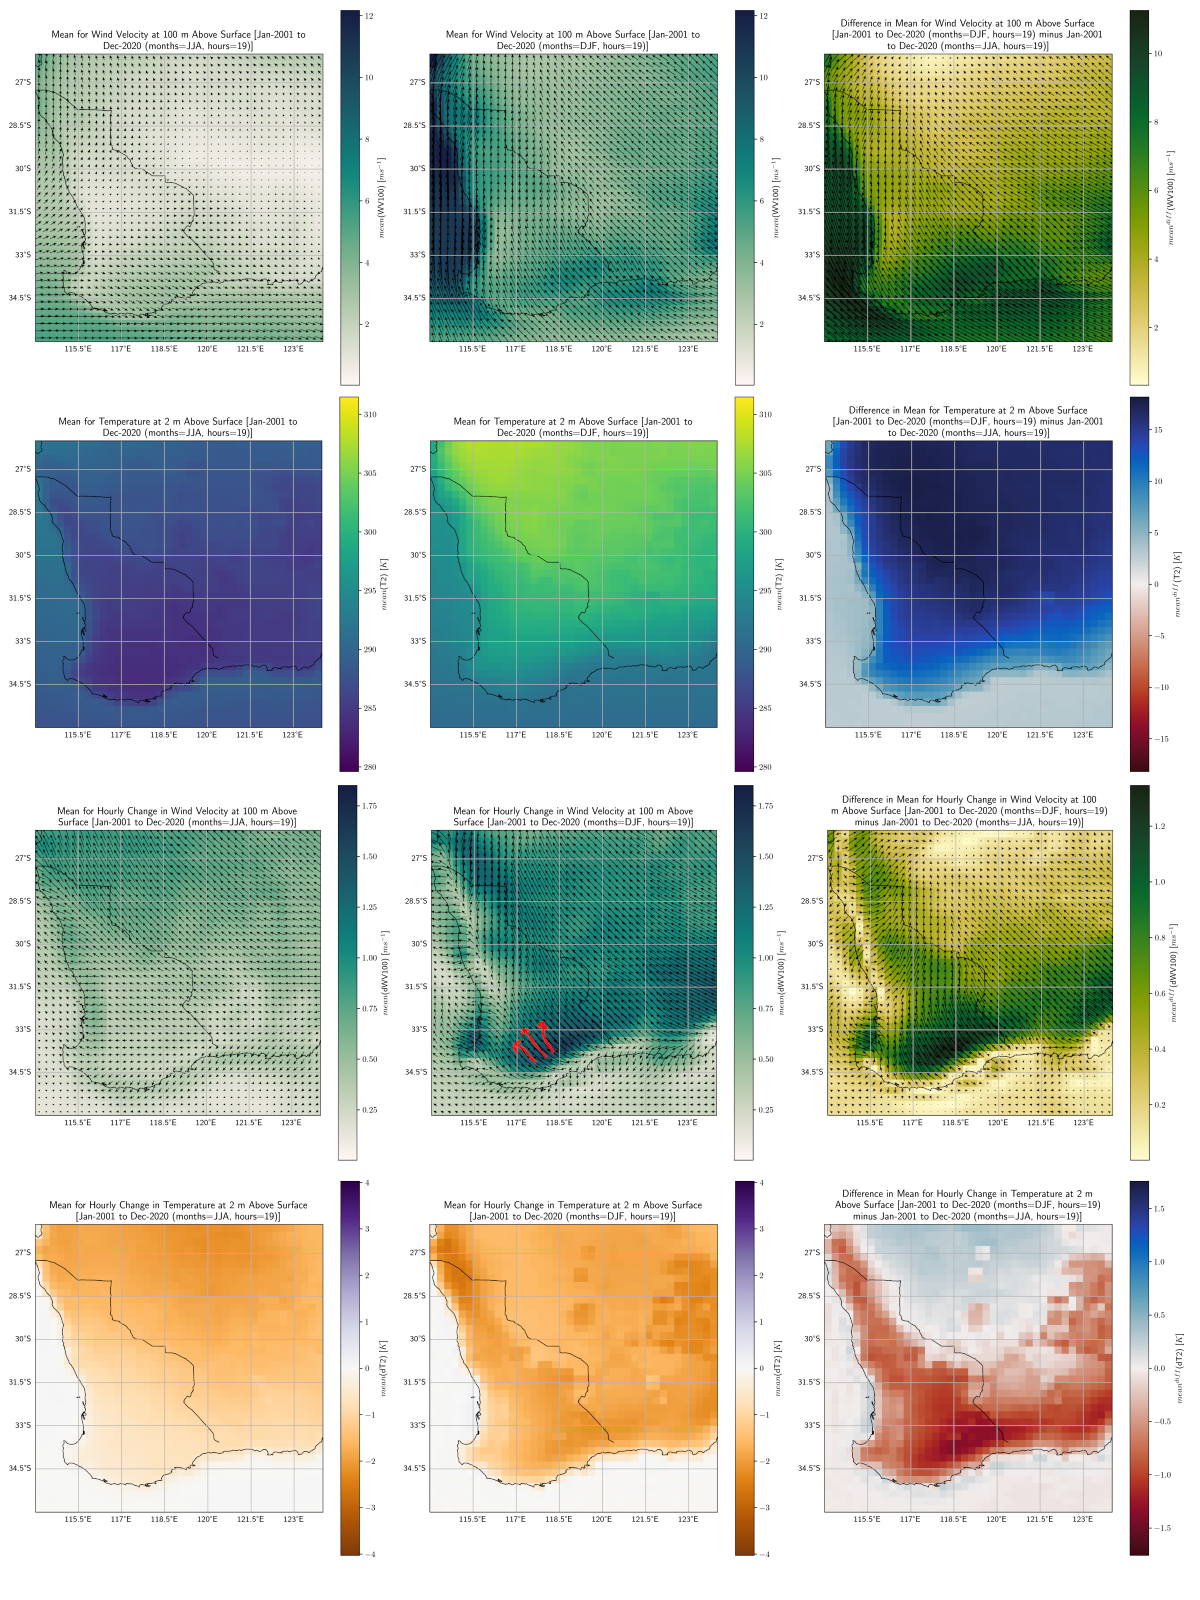
\includegraphics[width=0.9\textwidth]{wa_19_comb.png}
	\caption[Divergent wind changes during evening]{1900 mean \ac{JJA} and \ac{DJF} values for \acs{WV100}, \acs{T2}, \acs{dWV100} and \acs{dT2}. Red arrows (exaggerated) highlight the divergence in hourly wind changes. Magnitude of \ac{dWV100} near northern part of fence is higher than nearby coast despite weaker contrast in \ac{dT2}.}
	\label{fig:wa_19_comb}
\end{figure}

\paragraph{Modulation of convergence}

That is, there is a component of energy exchange flux across the fence, as well as a component of the moisture convergence flux towards the fence displayed in Figure~\ref{fig:wa_vidmf}, which appears to occur in a direction \textit{perpendicular} to that of the prevailing wind direction. In this picture, the native vegetation is not necessarily increasing moisture convergence on the native side of the fence by drawing winds directly to itself, but rather it does so by modulating where atmospheric convergence (reflected by effects on \ac{VIEC}) occurs so that there is a flux of localised mass density changes across the fence.

\paragraph{Possible evidence for CIAD}

A further observation is that the magnitude of \ac{dWV100} in \ac{DJF} near the northern part of fence is higher than that at the nearby coast despite there being a weaker contrast in \ac{dT2}. So delineations of temperature change along the fence alone appear unable to account for the observed patterns, especially since higher elevations on the native side of the fence (see Figure~\ref{fig:wa_orog}) imply a weakening agricultural breeze during the evening transition on top of this. But these results would be consistent under the \ac{CIAD} framework due to atmospheric condensation during the evening transition causing a decrease in pressure on the native side of the fence. Hourly means analysis for \ac{NAC} does indeed show a local maximum around the  evening transition (not shown) but results are confounded by assimilation cycle artefacts in \ac{ERA5} (see Appendix~\ref{sec:artefact}).

\subsection{Direct link between native vegetation and NAC}
\label{ssec:native_nac}

\subsubsection{Clouds prefer native vegetation, in summer}

Studies by \citet{lyons1993, lyons1996, lyons2002, ray2003, nair2011} already clearly demonstrate the sensitivity of cloud formation to type of vegetation cover (see Figure~\ref{fig:cloud_satellite}), and argue this is the result of differences in surface heat flux partitioning causing differences in boundary layer thickness.

\ac{MDP} means for \ac{DJF} in Figure~\ref{fig:wa_stats_seasonal_2} display significantly greater values for \ac{SSHF}, \ac{BLH} and \ac{NAC} on the native side of the fence, with sharp delineation at the fence (and these appear to arise from lower albedo), giving further support to these authors' arguments and the notion that "clouds prefer native vegetation" \citep{lyons2002} (at least in summer).

\begin{figure}[!htp]
	\centering
	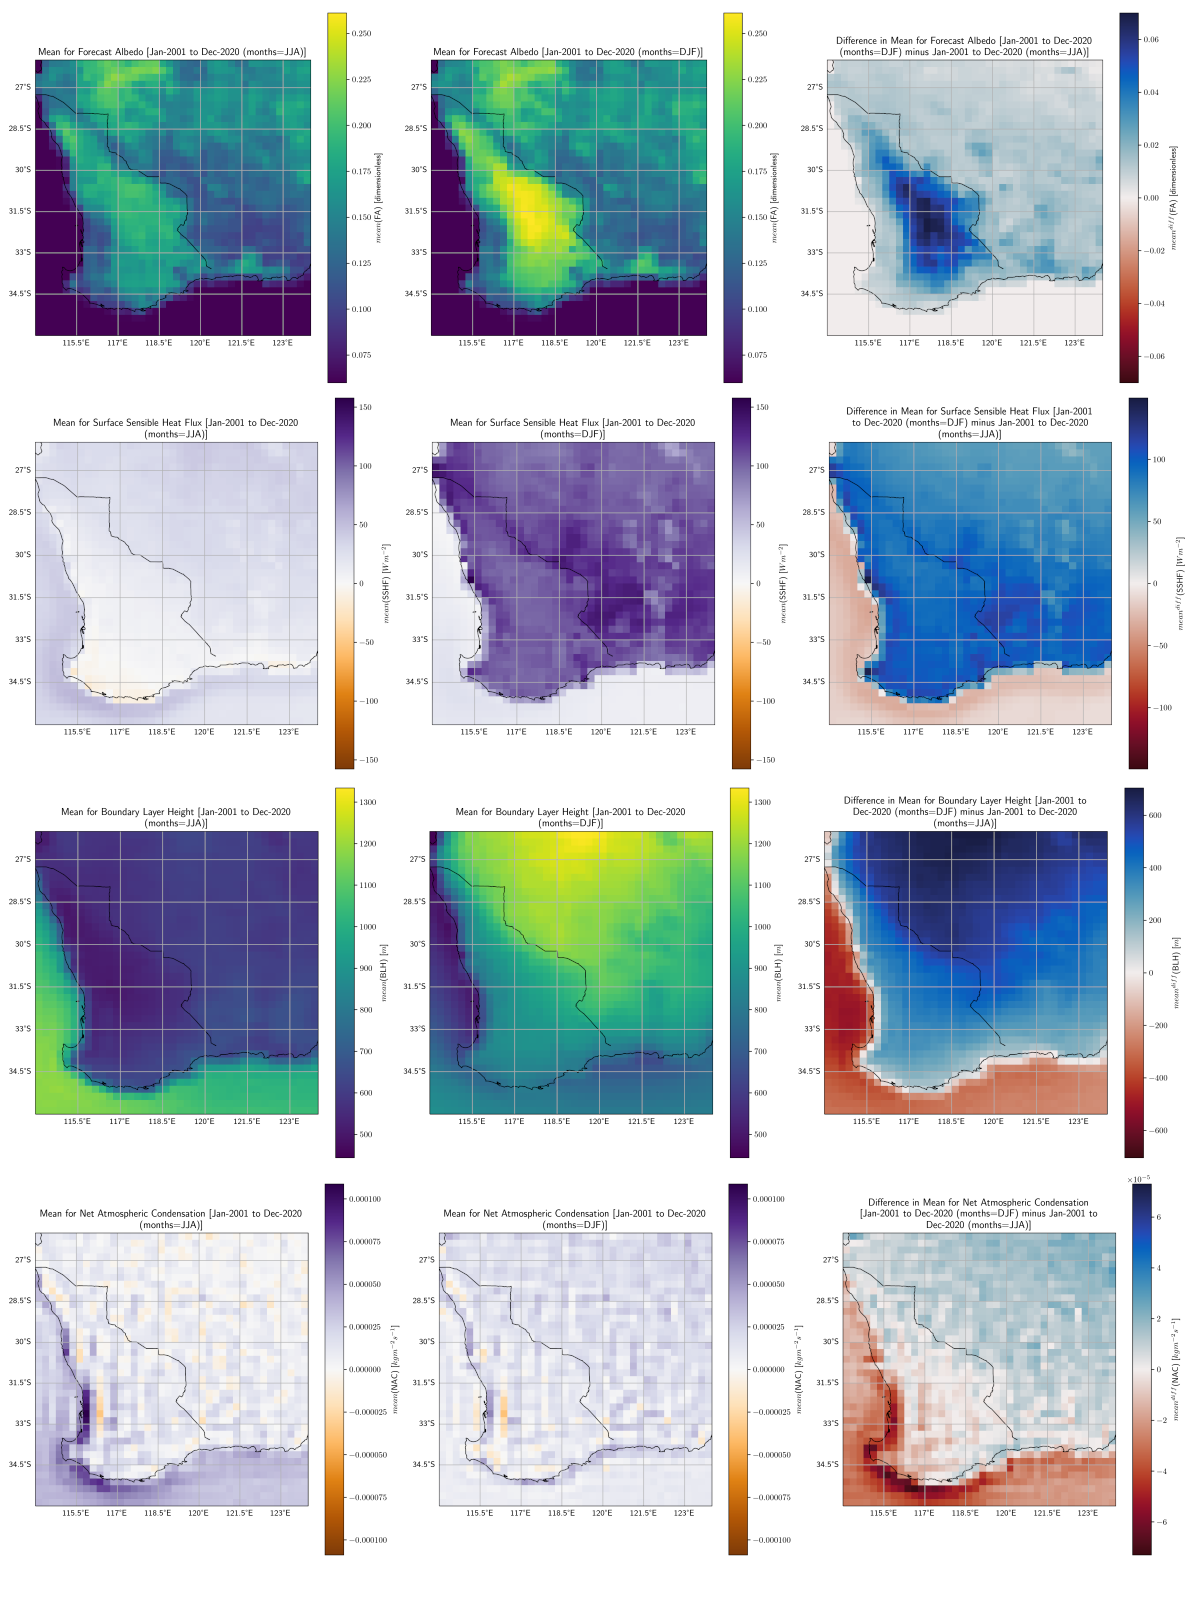
\includegraphics[width=0.9\textwidth]{wa_stats_seasonal_2.png}
	\caption[Selected MDP means with fence delineations]{\acs{MDP} means for \acs{FA}, \acs{SSHF}, \acs{BLH} and \acs{NAC} illustrate how the lower albedo of native vegetation leads to a thicker boundary layer via increased sensible heat for convective mixing, which in turn promotes increased atmospheric condensation (cloud formation).}
	\label{fig:wa_stats_seasonal_2}
\end{figure}

\subsubsection{Other contributions to NAC}

However, this may not be the full picture as the trends for \ac{SSHF}, \ac{BLH} and \ac{NAC} do not fully correlate with each other. \ac{BLH} appears to also be correlated with \ac{LSE} (compare with Figure~\ref{fig:wa_orog}) and this may possibly arise from wind shear effects.

\ac{CCN} particle size distributions resulting from native vegetation \ac{VOC} release forming \ac{SOA} may also affect \ac{NAC} patterns. Hourly means analysis reveals that night time condensation on the native side of the fence for \ac{DJF} is slightly higher than on the agricultural side of the fence, even when \ac{SSHF} is practically the same on both sides. If the \ac{CIAD} framework is valid, then another possible contribution is that moisture advection towards the native side of the fence (as observed in Figure~\ref{fig:wa_vidmf}) may then have a domino effect in making condensation further west of the fence more likely.

\subsubsection{Revisiting causation between VIEC and NAC}

Throughout the analysis of our results, we have turned to the question of whether positive \ac{NAC} (cloud formation) is primarily the result of negative \ac{VIEC} (rising air) or whether it is other way around (in line with the framework of \ac{CIAD}). Given that more positive \ac{NAC} in large part appears to directly result from surface energy balance effects, it calls into question yet again what additional causation \ac{VIEC} might have on top of this.

\paragraph{Contribution from SSHF}

There is very limited causation from \ac{VIEC} to \ac{SSHF} since the former is an atmospheric process and the latter is mostly a surface effect. So the remaining argument against \ac{CIAD} is either that \ac{SSHF} (perhaps in confluence with topography) produces the observed uplift of air masses which then leads to condensation (i.e.\ \ac{VIEC} is an intermediate cause between \ac{SSHF} and \ac{NAC}), or that \ac{SSHF} simultaneously causes similar patterns in \ac{VIEC} and \ac{NAC} via separate mechanisms (i.e.\ \ac{SSHF} is a confounding factor leading to a spurious correlation between \ac{VIEC} and \ac{NAC}).

\paragraph{SSHF alone cannot account for VIEC}

But neither of these seem to be the case because while the correlation between \ac{VIEC} and \ac{NAC} continues to hold during the \ac{JJA} months, hourly means analysis reveals that \ac{SSHF} actually displays the opposite trend to these variables as it does in \ac{DJF}. That is, \ac{SSHF} during \ac{JJA} is suppressed over agricultural land due to irrigation of crops, but all the while there is increased condensation with a very likely cause from increased evapotranspiration, and there is a correlated change to more \textit{negative} \ac{VIEC} values (more uplift) despite the \textit{decreased} \ac{SSHF}. Analogous results also apply on the native side of the fence with decreased evapotranspiration from native plants during \ac{JJA}. Furthermore, \ac{SSHF} is not at all correlated with any of the coastal effects observed in \ac{JJA} (see Section~\ref{ssec:coastal_cond}).

In summary, the idea that \ac{NAC} plays a causative role in \ac{VIEC} (possibly then leading to feedback) appears better supported by the available evidence than the idea that \ac{NAC} is a passive result of \ac{VIEC}.

\section{Similar comparison}

\subsection{Study periods}

\subsubsection{Selected periods}

For \ac{WA}, the selected periods for the similar comparison was from Jun-1997 to May-2002 and from Sep-2010 to Aug-2015 (see Figure~\ref{fig:wa_ind}). 

\begin{figure}[!ht]
	\centering
	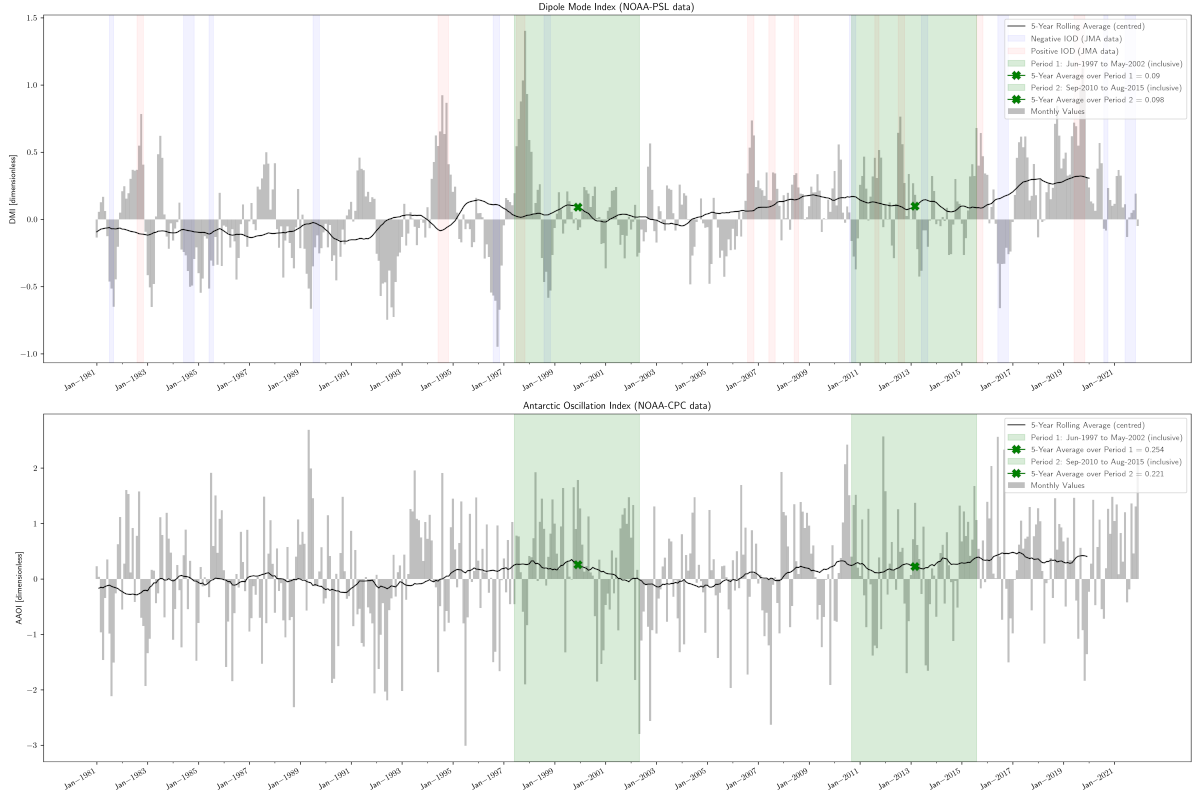
\includegraphics[width=0.9\textwidth]{wa_ind.png}
	\caption[WA's relevant climate indices for similar comparison]{\ac{NOAA} climate indices for climate drivers in \ac{WA}. Green shading highlights selected periods. Blue and red shading highlight negative and positive \ac{IOD} events respectively.}
	\label{fig:wa_ind}
\end{figure}

Between these periods was extensive vegetation loss concentrated along the coastal forests (see Figure~\ref{fig:wa_lai_similar}), resulting from a mix of drought events and human activities such as mining and forestry (beyond vegetation clearing, these activities are also implicated in causing a drop in the region's water table \citep{gordon2003, bauxite_hydro, johnson2003}).

\begin{figure}[!ht]
	\centering
	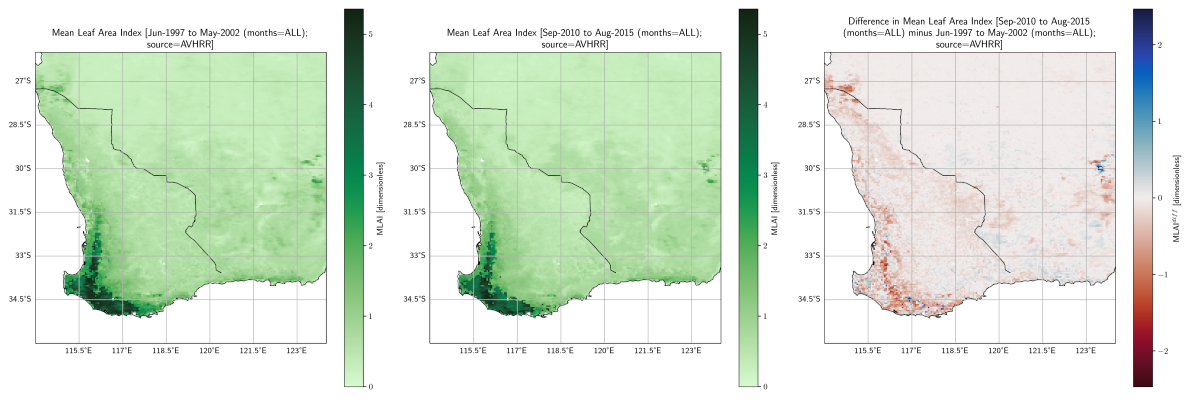
\includegraphics[width=0.9\textwidth]{wa_lai_similar.png}
	\caption[MLAI similar comparison for WA focus region]{\ac{MLAI} computed over each period in the similar comparison (left and middle), as well as the difference in these values between the two periods (right).}
	\label{fig:wa_lai_similar}
\end{figure}

\subsubsection{Comparable values in climate indices}

The main climate drivers for this region are the \ac{IOD} and \ac{AAO} (also known as \ac{SAM}) \citep{wa_drivers}. The corresponding indices are the \ac{DMI} and \ac{AAOI} respectively, and these = have similar averages over these periods. In fact, the 5-year averages over all the indices apart from the \ac{EPOI} (which is distant and not expected to have significant effects\footnote{Significant effects from teleconnections are possible but we have assumed this isn't the case here}.) have very similar values (not shown), although they appear to span across different phases for the longer-term oscillations.

\subsubsection{Summary of IOD events}

The period from Jun-1997 to May-2002 contains one Negative \ac{IOD} event and one Positive \ac{IOD} event, both of which display relatively high magnitudes for monthly values. Although the period from Sep-2010 to Aug-2015 contain two Negative \ac{IOD} events and two Positive \ac{IOD} events, each of these display relatively low magnitude in monthly values and so should still be comparable against the first period.

\subsection{Findings}
\label{ssec:similar_find}

No obviously remarkable correlations with coastal \ac{MLAI} loss was observed. Occasional delineations along forest cover did occur, but were too inconsistent to rule out the possibility of spurious relationships. It was also difficult to distinguish whether the occasional trends resulted from coastal \ac{MLAI} loss or modulation of atmospheric differences by the coast itself. However, sharp delineations along the fence are observed again in \ac{JJA} \ac{MDP} statistics despite minimal \ac{MLAI} loss around here, indicating that land cover imposes a local modulation upon changes in the synoptic background.

A change in \ac{JJA} synoptic conditions between periods sees an increase of \ac{MSLP} through the region despite increased \ac{T2}. The \ac{MSLP} increase in the northern part of the focus region is especially weak due to being offset by increased temperatures (especially on the native side of the fence). There is increased cloud formation (positive \ac{NAC}$^{diff}$) in subregions on the native side of the fence despite the increase in surface pressure. As with previous results, more positive \ac{NAC}$^{diff}$ correlates with more negative \ac{VIEC}$^{diff}$. \ac{VIEC}$^{diff}$, \ac{NAC}$^{diff}$ and \ac{VIDMF}$^{diff}$ all show sharp distinctions along the fence, with increased moisture convergence on the native side of the fence. See Figure~\ref{fig:wa_stats_similiar_1}.

While agricultural crops continued to transpire under the drier conditions, native vegetation reduced its transpiration, with a sharp decrease in its \ac{MDP} maximum. This in turn led to dramatic fence delineations in the \ac{MDP} maximum and minimum for \ac{NAC}, although this is partially confounded by \ac{ERA5} assimilation cycle artefacts (see Appendix~\ref{sec:artefact}). $range$(\ac{VIKE}) for \ac{JJA} continued to show delineation along the fence, but less so along the coastal forests, and a delineation is observed in the hour of \textit{minimum} rather than maximum. It is not clear what causes these \ac{VIKE} effects. See Figure~\ref{fig:wa_stats_similiar_2}.

%\enlargethispage{\baselineskip} % so you do not get a single line in another page